%! Author = Omar Iskandarani
%! Title = A Topological Reformulation of the Standard Model via Vortex Æther Dynamics
%! Date = May 23, 2025
%! Affiliation = Independent Researcher, Groningen, The Netherlands
%! License = CC-BY 4.0
%! ORCID = 0009-0006-1686-3961

\documentclass[a4paper, aps,preprint,superscriptaddress, 12pt]{revtex4}
\usepackage[a4paper, margin=2cm]{geometry}
\usepackage{bookmark}
\usepackage{float}
\usepackage{tikz}
\usepackage{makecell}
\usepackage{tabularx}
\usepackage[font=footnotesize]{caption}
\usetikzlibrary{arrows.meta}
\usepackage{pgfplots}
\pgfplotsset{compat=1.18}
\usepackage[none]{hyphenat}
\usepackage{array}
\usepackage{amsmath}
\usepackage{booktabs}
\usepackage[utf8]{inputenc}
\usepackage{amssymb}
\usepackage{graphicx}
\usepackage{hyperref}
\usepackage{physics}
\usepackage{natbib}
\usepackage{url}
\usepackage{multirow}
\usepackage{subcaption}
\usepackage{siunitx}
\usepackage{listings}
\usepackage{lscape}
\renewcommand{\arraystretch}{1.5}
\renewcommand{\floatpagefraction}{.8}
\sloppy

\begin{document}

\author{Omar Iskandarani}
\title{A Topological Reformulation of the Standard Model via Vortex Æther Dynamics}
\date{Mei 2025}
\affiliation{Independent Researcher, Groningen, The Netherlands}
\thanks{ORCID: \href{https://orcid.org/0009-0006-1686-3961}{0009-0006-1686-3961}}
\email{info@omariskandarani.com}

\begin{abstract}
We present a reformulation of the Standard Model Lagrangian within the dimensional and topological framework of the Vortex Æther Model (VAM). In this approach, conventional quantum field terms are reinterpreted via fluid-mechanical analogs: particles correspond to knotted vortex excitations in a compressible æther, while interactions arise from swirl dynamics, circulation, and density fluctuations. The model replaces Planck-based constants with a complete set of natural units derived from mechanical quantities such as core radius (\(r_c\)), swirl velocity (\(C_e\)), and maximum æther force (\(F^\text{vam}_\text{max}\)). Coupling constants including \(\alpha\), \(\hbar\), and \(e\) emerge from vortex properties rather than being fundamental inputs. We show that gauge fields arise from swirl structure, fermionic behavior from knotted helicity propagation, and mass from internal topological tension rather than spontaneous symmetry breaking. The resulting Lagrangian is dimensionally self-consistent, with all dynamics and interactions geometrically and physically grounded. This framework provides a unified mechanical ontology for quantum fields and offers new insights into the origins of mass, charge, and time from first principles.
\end{abstract}

    \maketitle

    \section{Introduction}\label{sec:inleiding}

Despite the empirical success of the Standard Model (SM) of particle physics and General Relativity (GR), fundamental questions remain unresolved: What is the physical origin of mass? Why do gauge interactions exhibit their particular symmetries? What gives rise to natural constants such as $\hbar$, $e$, or $\alpha$ beyond dimensional convenience?

Mainstream physics relies heavily on abstract mathematical formalisms—such as symmetry groups, Lagrangian terms, and quantum operators—that, while predictive, often obscure the underlying physical ontology. This paper proposes an alternative: the \emph{Vortex Æther Model} (VAM), a mechanistic, fluid-dynamic framework in which spacetime and all physical phenomena emerge from structured motion in a compressible, superfluid-like æther.

In VAM, elementary particles are not point-like fields but stable, knotted vortex structures embedded in the æther. Observable properties such as mass, charge, spin, and flavor are reinterpreted as topological and dynamical characteristics—circulation strength, core radius, swirl helicity—of these vortex knots. Gauge and Higgs interactions are expressed as manifestations of fluid tension, reconnection, and swirl transfer.

Crucially, this is not merely a reformulation of mathematical symbols. The goal of VAM is to provide an \emph{ontological replacement} for conventional quantum field theory: a physically intuitive, testable substrate from which all constants and couplings emerge. Within this framework, the Standard Model is reconstructed from five physically meaningful ætheric quantities: swirl velocity $C_e$, core radius $r_c$, æther density $\rho_\text{\ae}$\footnote{The VAM framework distinguishes between three æther densities depending on context: fluid, energy, and mass-equivalent. See Table~\ref{tab:ae_densities_foot} for a breakdown of these definitions. A mismatch in interpretation leads to inconsistencies in field derivations.}, maximum force $F^{\text{max}}_{\text{\ae}}$, and circulation $\Gamma$.

This paper presents a full reformulation of the Standard Model Lagrangian using these VAM-derived units and fields. Each term acquires a mechanical and geometric interpretation, leading to a unified description where quantum phenomena, gauge structures, and mass generation are consequences of vortex dynamics in an inviscid æther. A full field-theoretic derivation of the model dynamics is presented in Appendix~\ref{sec:EL-derivation}.

Historically, this effort revives foundational ideas from Kelvin's vortex-atom hypothesis and Maxwell's æther mechanics, updating them within a modern context informed by quantum fluids, superfluid analogs of gravity, and topological field theory. See, for example, Volovik's emergent gravity framework in helium II~\cite{Volovik2003UniverseInHelium}, Barceló et al.'s review of analog spacetime geometries~\cite{Barcelo2005AnalogueGravityReview}, and Kleckner and Irvine's experimental realization of knotted vortices~\cite{Kleckner2013KnottedVortices}. While this paper is designed to be standalone, these works contextualize the broader landscape of fluid-based physical models.

By grounding the abstract structures of modern physics in vortex geometry, VAM aims to bridge the gap between formal theory and intuitive physical mechanisms—offering not only reinterpretation, but a re-foundation of particle physics itself.

This work builds on a series of earlier papers developing the Vortex Æther Model (VAM). In \cite{iskandarani2025timedilation}, proper time was defined through internal angular motion of vortex cores, introducing the concept of \("\)swirl clocks\("\) as the microscopic origin of time dilation. This was extended in \cite{iskandarani2025swirlgravity}, which proposed that gradients in swirl clocks — arising from non-uniform vorticity — mimic gravitational curvature, including analogs to event horizons. The present work synthesizes these concepts into a variational field-theoretic framework, reformulating the Standard Model Lagrangian in terms of helicity, core structure, and topological æther dynamics.

\subsection*{Postulates of the Vortex Æther Model}
\begin{table}[h!]
    \centering
    \begin{tabular}{rl}
        \hline
        \textbf{1. Continuous Space} & Space is Euclidean, incompressible and inviscid. \\
        \textbf{2. Knotted Particles} & Matter consists of topologically stable vortex nodes. \\
        \textbf{3. Vorticity} & The vortex circulation is conserved and quantized. \\
        \textbf{4. Absolute Time} & Time flows uniformly throughout the æther. \\
        \textbf{5. Local Time} & Time is locally slower due to pressure and vorticity gradients. \\
        \textbf{6. Gravity} & Emerges from vorticity-induced pressure gradients. \\
        \hline
        \bottomrule
    \end{tabular}
    \caption{Postulates of the Vortex Æther Model (VAM).}
    \label{tab:postulates}
\end{table}

The postulates replace spacetime curvature with structured rotational flows and thus form the foundation for emergent mass, time, inertia, and gravity.

\section*{Terminology and Classical Correspondence}

We introduce several novel constructs to describe the vortex-based field framework. For clarity, Table~\ref{tab:vam_definitions} provides precise definitions and links to standard physics concepts.

\begin{table}[H]
    \centering
    \scriptsize
    \renewcommand{\arraystretch}{1.3}
    \begin{tabular}{|l|l|l|}
        \hline
        \textbf{Term} & \textbf{Definition in VAM} & \textbf{Analogy in Established Theory} \\
        \hline
        \makecell[l]{Swirl Clock} &
        \makecell[l]{Proper time defined by internal angular frequency \\ $\omega_0$ of a vortex core} &
        \makecell[l]{Atomic clock (GR); spin-precession \\ in gyroscopes} \\
        \hline
        \makecell[l]{Swirl Lagrangian} &
        \makecell[l]{Field Lagrangian including helicity term \\ $\lambda (\mathbf{v} \cdot \boldsymbol{\omega})$} &
        \makecell[l]{Chern–Simons terms; \\ topological terms in QFT} \\
        \hline
        \makecell[l]{Helicity Time} &
        \makecell[l]{Clock rate modulated by helicity density: \\ $d\tau \propto \mathbf{v} \cdot \boldsymbol{\omega}$} &
        \makecell[l]{Phase evolution in rotating frames; \\ action-angle methods} \\
        \hline
        \makecell[l]{Core Radius $r_c$} &
        \makecell[l]{Characteristic radius of maximal vorticity \\ and core energy density} &
        \makecell[l]{Healing length in BECs; \\ flux tube radius in QCD} \\
        \hline
        \makecell[l]{Swirl Speed $C_e$} &
        \makecell[l]{Tangential speed of æther flow \\ at core radius} &
        \makecell[l]{Sound speed in superfluids; \\ Lorentz frame velocity} \\
        \hline
        \makecell[l]{Swirl Horizon} &
        \makecell[l]{Boundary beyond which $\omega_{\text{obs}} \to 0$ \\ and clocks stall} &
        \makecell[l]{GR event horizon; \\ ergosphere boundary (Kerr geometry)} \\
        \hline
    \end{tabular}
    \caption{Key theoretical constructs in the Vortex Æther Model (VAM), mapped to classical and quantum analogs for interpretability.}
    \label{tab:vam_definitions}
\end{table}


These constructs provide an intuitive bridge between fluid mechanics, quantum field theory, and emergent spacetime phenomena, facilitating reinterpretation of the Standard Model Lagrangian in a vortex-based æther framework.
    \section{Motivation}

The Standard Model Lagrangian is one of the most successful constructs in modern physics, unifying electromagnetic, weak, and strong interactions within a renormalizable quantum field theory. Yet it remains structurally incomplete in a physical sense: its mass terms, symmetry groups, and coupling constants are introduced \textit{a priori}, without geometric or mechanical derivation.

For instance, the fine-structure constant $\alpha \approx 1/137$ appears as an empirical ratio with no explanation for its value. The elementary charge $e$ and Planck constant $\hbar$ are similarly inserted into the theory to match experimental outcomes, but have no origin within the theory’s own framework. Even the Higgs vacuum expectation value (VEV), essential for mass generation, is externally imposed rather than derived.

The Vortex Æther Model (VAM) addresses these gaps by reconstructing the Standard Model from the ground up using topologically and mechanically grounded vortex structures. Rather than assuming discrete point particles and abstract quantum fields, VAM postulates a compressible, rotating æther medium in which all elementary particles are topologically stable vortex knots. Their observable properties—mass, charge, spin, and even local time—emerge from measurable fluidic parameters such as circulation strength, core radius, helicity, and swirl velocity.

In this framework, constants such as $\alpha$ and $\hbar$ are not arbitrary. For example, $\alpha$ is shown to emerge from the swirl geometry of the æther via the dimensionless ratio $\alpha = 2C_e / c$, while $\hbar$ is interpreted as a manifestation of quantized circulation within a vortex structure. These reconstructions offer not only physical intuition, but also potential explanations for why such constants take the values they do. A summary comparison is presented in Table~\ref{tab:SM_vs_VAM_constants}, contrasting key constants across both frameworks.

This approach aligns with principles established in superfluid dynamics, topological field theory, and analog gravity systems. By expressing Standard Model terms in VAM units and connecting abstract constants to physical flow properties, the model opens pathways to new testable predictions—particularly regarding vacuum energy, neutrino mass generation, and mechanisms of quark confinement.



\subsection*{Unified Constants and Units in VAM}

The table below summarizes the complete set of mechanical and topological quantities used throughout the Vortex Æther Model. These values form a self-contained replacement for Planck-based dimensional analysis.


\begin{table}[H]
    \centering
    \footnotesize
    \renewcommand{\arraystretch}{1.3}
    \begin{tabular}{|l|l|l|l|}
        \hline
        \textbf{Symbol} & \textbf{Formula / Definition} & \textbf{Interpretation in VAM} & \textbf{Approx. Value (SI)} \\
        \hline

        $C_e$ &
        — &
        Core swirl velocity; sets intrinsic time rate of particles &
        $1.094 \times 10^6$ m/s \\
        \hline

        $r_c$ &
        — &
        Radius of vortex core; spatial extent of a particle &
        $1.409 \times 10^{-15}$ m \\
        \hline

        $\rho_\text{\ae}$ &
        — &
        Æther density; determines flow inertia and stress limits &
        $3.893 \times 10^{18}$ kg/m³ \\
        \hline

        $F^{\text{vam}}_\text{max}$ &
        $\pi r_c^2 C_e \rho_\text{\ae}$ &
        Max transmissible force through æther (vortex core tension) &
        $\sim 29.05$ N \\
        \hline

        $F^{\text{gr}}_\text{max}$ &
        $\frac{c^4}{4G}$ &
        GR-based theoretical maximum force limit &
        $\sim 3.0 \times 10^{43}$ N \\
        \hline

        $\kappa$ &
        $\frac{\Gamma}{n}$ or quantized $\oint \vec{v} \cdot d\vec{\ell}$ &
        Quantum of circulation per vortex loop &
        $1.54 \times 10^{-9}$ m²/s \\
        \hline

        $\alpha$ &
        $\frac{2 C_e}{c}$ &
        Fine-structure constant from swirl-to-light ratio &
        $7.297 \times 10^{-3}$ (unitless) \\
        \hline

        $t_P$ &
        $\frac{r_c}{c}$ &
        Fastest rotation cycle (Planck time analog) &
        $\sim 5.39 \times 10^{-44}$ s \\
        \hline

        $\Gamma$ &
        $\oint \vec{v} \cdot d\vec{\ell}$ &
        Total circulation; encodes angular momentum &
        (typical unit: m²/s) \\
        \hline

        $t$ &
        $dt \propto \frac{1}{\vec{v} \cdot \vec{\omega}}$ &
        Local time rate derived from helicity field configuration &
        (unit: s) \\
        \hline

        $\mathcal{H}_\text{topo}$ &
        $\int \vec{v} \cdot \vec{\omega} \, dV$ &
        Topological helicity; measures vortex alignment &
        (unit: m³/s²) \\
        \hline
    \end{tabular}
    \caption{Fundamental parameters in the Vortex Æther Model (VAM). These quantities form the physical and topological basis for mass, time, charge, and quantum behavior. Each is experimentally meaningful and derivable from ætheric flow geometry.}
    \label{tab:VAM_master_table}
\end{table}


\subsection*{Derived Couplings and Constants in VAM}
From the core æther parameters introduced above, several familiar physical constants can be re-expressed as derived quantities. These include the Planck constant, the speed of light, the fine-structure constant, and the elementary charge—all reconstructed as emergent properties of swirl and circulation. Table~\ref{tab:VAM_master_table} summarizes these reformulations.

Within VAM, the maximum vortex interaction force is derived explicitly from Planck-scale physics:
\begin{equation}
    F^{\text{vam}}_\text{max} = \alpha \left(\frac{c^4}{4G}\right)  \left(\frac{r_c}{l_p}\right)^{-2}
\end{equation}

where $\frac{c^4}{4G}$ is the Maximum Force in nature $F^{\text{gr}}_\text{max}$, the stress limit of the æther found from General Relativity, and $l_p$ is the Planck Length.


\subsection*{Comparative Origins of Constants: Standard Model vs. VAM}

The re-expression of fundamental constants within VAM highlights a key philosophical and physical distinction: while the Standard Model treats quantities like $\alpha$, $\hbar$, and $e$ as empirical inputs, the Vortex Æther Model derives them from topological and geometric features of the æther flow.

The table below contrasts how key constants are introduced or derived in both frameworks.

\begin{table}[H]
    \centering
    \footnotesize
    \renewcommand{\arraystretch}{1.3}
    \begin{tabular}{|l|l|l|}
        \hline
        \textbf{Constant} & \textbf{Standard Model Treatment} & \textbf{VAM Derivation / Interpretation} \\
        \hline
        \makecell[l]{Fine-Structure \\ Constant $\alpha$} &
        \makecell[l]{Empirical dimensionless constant \\ for EM interaction strength} &
        \makecell[l]{Emerges from swirl ratio: \\ $\alpha = \frac{2 C_e}{c}$; purely geometric} \\
        \hline

        \makecell[l]{Planck Constant \\ $\hbar$} &
        \makecell[l]{Postulated quantum of action; \\ enters commutation rules} &
        \makecell[l]{Circulation-induced impulse: \\ $\hbar \sim \rho_\text{\ae} \Gamma r_c^2$} \\
        \hline

        \makecell[l]{Elementary \\ Charge $e$} &
        \makecell[l]{Input coupling in QED \\ with no internal structure} &
        \makecell[l]{Swirl flux through vortex core: \\ $e \sim \rho_\text{\ae} C_e r_c^2$} \\
        \hline

        \makecell[l]{Speed of \\ Light $c$} &
        \makecell[l]{Postulated invariant limit \\ in SR and GR} &
        \makecell[l]{Calibration limit; \\ signal speed is $C_e < c$ \\ (Lorentz symmetry is emergent)} \\
        \hline

        \makecell[l]{Higgs VEV \\ $v$} &
        \makecell[l]{Free symmetry-breaking scale; \\ not derived internally} &
        \makecell[l]{Ætheric tension amplitude: \\ $v \sim \sqrt{F_\text{max}/\rho_\text{\ae}}$} \\
        \hline

        \makecell[l]{Maximum \\ Force $F_\text{max}$} &
        \makecell[l]{Rare in SM; from GR: \\ $F = c^4/4G$ in limit cases} &
        \makecell[l]{Derived from vortex tension: \\ $F_\text{max}^{\text{vam}} = \pi r_c^2 C_e \rho_\text{\ae}$} \\
        \hline
    \end{tabular}
    \caption{Ontological contrast between the Standard Model and the Vortex Æther Model regarding the origin of key physical constants. VAM replaces empirical insertions with mechanical derivations from swirl and æther geometry.}
    \label{tab:SM_vs_VAM_constants}
\end{table}

\section*{Foundational Contrasts: Constants and Particles in VAM vs. SM}

Beyond constants, the Standard Model also posits intrinsic properties of particles—mass, spin, charge, flavor—as axiomatic features of quantized fields. The Vortex Æther Model, by contrast, interprets these as emergent from topological and dynamic features of vortex structures in a rotating æther medium.
\begin{table}[H]
    \centering
    \footnotesize
    \renewcommand{\arraystretch}{1.3}
    \begin{tabular}{|l|l|l|}
        \hline
        \textbf{Particle Property} & \textbf{Standard Model Interpretation} & \textbf{VAM Interpretation} \\
        \hline
        \makecell[l]{Mass} &
        \makecell[l]{Introduced via Higgs field \\ with arbitrary Yukawa couplings} &
        \makecell[l]{Emergent from vortex inertia: \\ $m \propto \rho_\text{\ae} \Gamma / C_e$ \\ or tension within knotted core} \\
        \hline
        \makecell[l]{Spin} &
        \makecell[l]{Intrinsic angular momentum \\ ($\hbar/2$ for fermions)} &
        \makecell[l]{Topological twist of vortex core \\ (e.g., Möbius loop linking)} \\
        \hline
        \makecell[l]{Electric Charge} &
        \makecell[l]{Coupling to $U(1)$ gauge field; \\ conserved via symmetry} &
        \makecell[l]{Swirl flux through core: \\ $e \sim \rho_\text{\ae} C_e r_c^2$ \\ (sign from swirl handedness)} \\
        \hline
        \makecell[l]{Flavor (Generations)} &
        \makecell[l]{Empirically distinct; \\ no structural rationale} &
        \makecell[l]{Knot complexity or higher-order \\ toroidal mode excitations} \\
        \hline
        \makecell[l]{Color Charge} &
        \makecell[l]{$SU(3)$ triplet charges; \\ source of strong force} &
        \makecell[l]{Filament braiding states or \\ phase twist between vortices} \\
        \hline
        \makecell[l]{Antiparticles} &
        \makecell[l]{Charge-conjugated fields \\ with opposite quantum numbers} &
        \makecell[l]{Mirror vortices with opposite \\ helicity and circulation} \\
        \hline
        \makecell[l]{Mixing (CKM/PMNS)} &
        \makecell[l]{Unitary matrices for \\ mass eigenstate mixing} &
        \makecell[l]{Oscillations from vortex coupling \\ or internal torsion precession} \\
        \hline
    \end{tabular}
    \caption{Ontological contrast between the Standard Model and the Vortex Æther Model in explaining intrinsic particle properties. In VAM, each feature arises from topological structure and flow dynamics within the æther.}
    \label{tab:SM_vs_VAM_particles}
\end{table}




    \input{section/03_natural_æther_constants}
    \section{Reformulating the Standard Model Lagrangian in VAM Units}\label{sec:lagrangian_vam}
The Standard Model Lagrangian encapsulates particle dynamics through symmetry-based field terms:
\begin{equation}
    \mathcal{L}_{\text{SM}} = -\frac{1}{4}F^{\mu\nu}F_{\mu\nu} + i\bar{\psi}\gamma^\mu D_\mu \psi + y_f \bar{\psi}\phi \psi + |D_\mu \phi|^2 - V(\phi)
\end{equation}
While mathematically elegant, these terms are not derived from first physical principles but are inserted axiomatically. The Vortex Æther Model (VAM) replaces this abstraction with a Lagrangian based on vortex dynamics, æther strain, and helicity conservation.

\subsection*{Core Assumptions}
\begin{itemize}
    \item The æther is a compressible, barotropic superfluid with stable vortex excitations.
    \item Particles are topologically stable vortex knots with quantized circulation.
    \item The Euler–Lagrange formalism applies to the action integral over fluid kinetic and potential energy densities.
    \item Helicity and vorticity are conserved modulo reconnection events.
\end{itemize}

\subsection*{Remarks on Spacetime Treatment}

In this model, the action integral is expressed as:
\[
    S = \int dt \int_{\mathbb{R}^3} \mathcal{L}(\vec{v}, \Phi, \rho_\text{\ae}, \dots) \, d^3x,
\]
reflecting a 3+1 decomposition with \textbf{absolute Newtonian time} and \textbf{Euclidean spatial geometry}.

Unlike relativistic field theories defined on Minkowski space \( \mathbb{R}^{1,3} \), the VAM adopts a \textbf{non-relativistic ontology}, where time is globally ordered and external to field dynamics.

This approach is consistent with established non-relativistic field theories, such as the Gross–Pitaevskii and hydrodynamic models for Bose–Einstein condensates, where space and time are decoupled and the Lagrangian formalism operates over \( \mathbb{R}^3 \times \mathbb{R} \)~\cite{Pethick2008BEC}.

Relativistic invariance in this context is regarded as an \textbf{emergent symmetry} that may arise at large scales or in specific limits of vortex behavior.

\subsection*{VAM-Reformulated Lagrangian}
Each term in the SM Lagrangian maps to a mechanical analog:

\begin{align*}
    \mathcal{L}_\text{VAM} &= \underbrace{-\frac{1}{4} \sum_{a} W^{a}_{\mu\nu} W^{a\mu\nu}}_{\text{Gauge field vorticity}}
    + \underbrace{\sum_{f} i \, m_f C_e r_c \, \bar{\psi}_f \gamma^\mu D_\mu \psi_f}_{\text{Fermion swirl propagation}} \\
    &- \underbrace{|D_\mu \phi|^2}_{\text{Æther strain field}}
    - \underbrace{V(\phi)}_{\text{Æther compression potential}}
    - \underbrace{\sum_f y_f \bar{\psi}_f \phi \psi_f + \text{h.c.}}_{\text{Mass coupling}}
    + \underbrace{\mathcal{H}_\text{topo}}_{\text{Vortex helicity term}}
\end{align*}

Where:
\[
    V(\phi) = -\frac{F_\text{max}}{r_c}|\phi|^2 + \lambda |\phi|^4
    \quad \text{and} \quad \mathcal{H}_\text{topo} = \int \vec{v} \cdot \vec{\omega} \, dV
\]
The full variational derivation of this Lagrangian—including Euler–Lagrange equations for velocity, scalar, and density fields—is provided in Appendix~\ref{sec:EL-derivation}.

\subsection{Gauge Fields as Vorticity Structures}
From Helmholtz’s theorem, the energy density in a vortex field is:
\begin{equation}
    \mathcal{L}_{\text{swirl}} = \frac{1}{2} \rho_\text{\ae} \left( |\vec{v}|^2 + \lambda |\nabla \times \vec{v}|^2 \right)
\end{equation}
Here, $\vec{v}$ is swirl velocity; $\lambda$ captures æther compressibility. Incompressible flows correspond to pure gauge configurations ($\nabla \cdot \vec{v} = 0$), while compressible strains allow field strength analogs.

\begin{figure}[H]
    \centering
    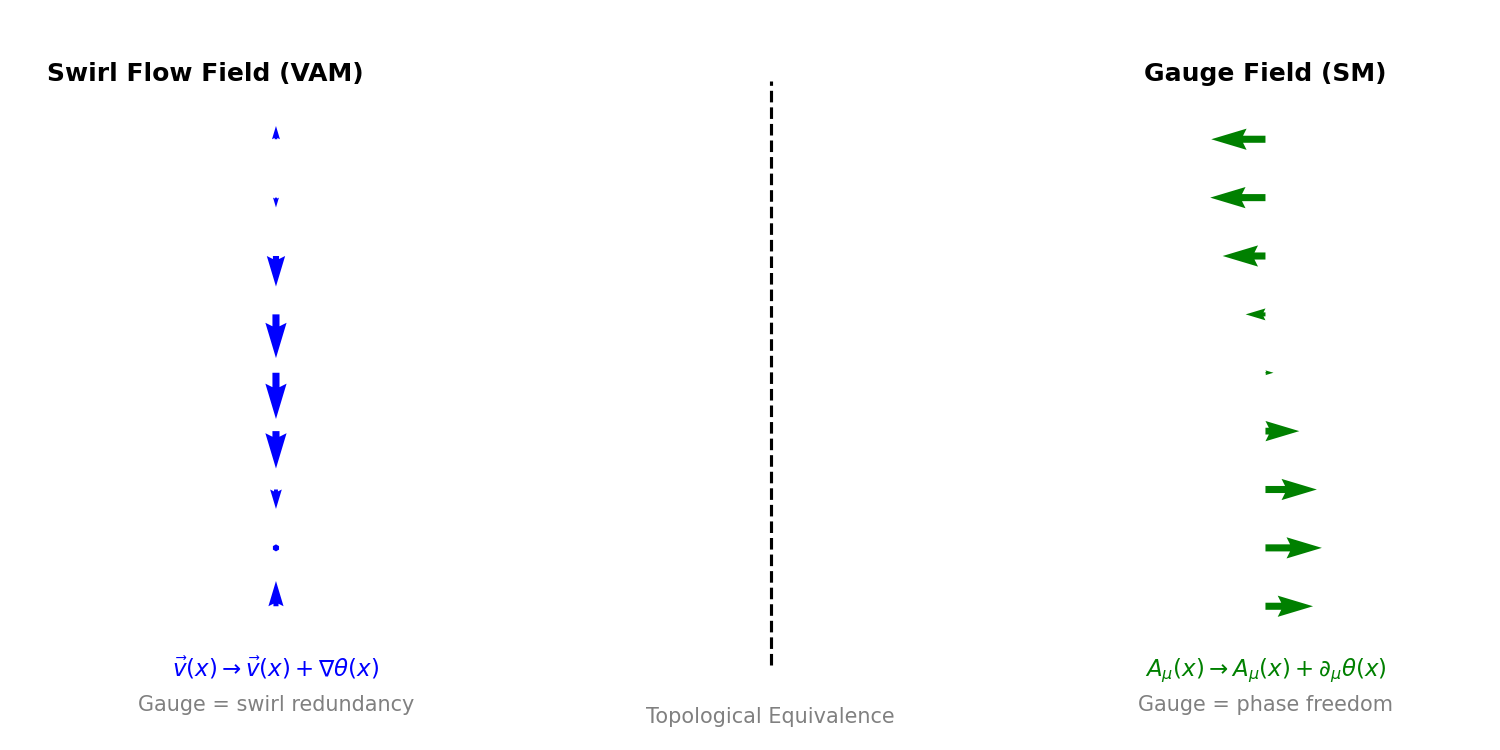
\includegraphics[width=0.95\textwidth]{gauge_swirl_equivalence}
    \caption{Analogy between gauge symmetry in the Standard Model and swirl invariance in the Vortex Æther Model (VAM). Both allow local reparameterizations that leave physical observables unchanged. Gauge symmetry in quantum field theory is structurally equivalent to potential-flow invariance in vortex dynamics.}
    \label{fig:gauge_swirl_equivalence}
\end{figure}

\begin{figure}[H]
    \centering
    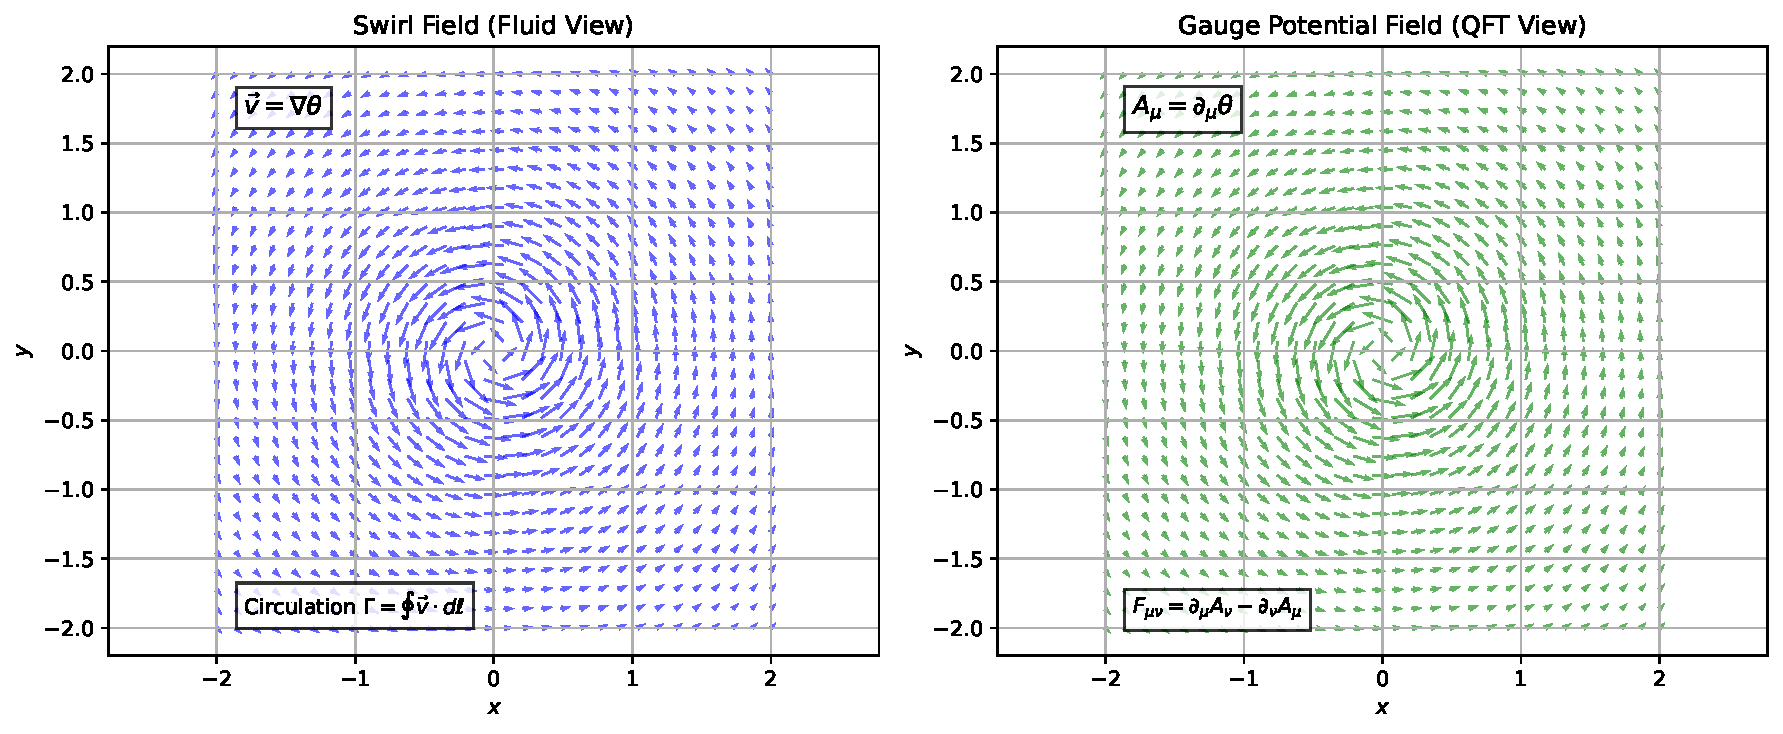
\includegraphics[width=0.9\linewidth]{SwirlVSGauge}
    \caption{
        Visual analogy between a fluid swirl field (left) and a gauge potential field in quantum field theory (right).
        Both fields depict circulation around a central core, but the left arises from mechanical vorticity in a compressible æther,
        while the right encodes electromagnetic or gauge interaction via abstract potential terms.
        This duality illustrates how local gauge invariance in QFT corresponds to conserved swirl topology in VAM.
    }
    \label{fig:swirl_gauge_analogy}
\end{figure}

\subsection{Fermion Kinetics via Swirl Propagation}
In the hydrodynamic formalism:
\begin{equation}
    \mathcal{L}_{\text{fermion}} = \rho_\text{\ae} C_e \Gamma \left( \psi^* \partial_t \psi - \vec{v} \cdot \nabla \psi \right)
\end{equation}
The convective derivative replaces $D_\mu$, and $\Gamma = 2\pi r_c C_e$ links to the particle’s spin-½ topology. Swirl modulates propagation analogous to minimal coupling.

\subsection{Mass from Helicity and Inertia}
The VAM mass term derives from vortex inertia under æther drag:
\begin{equation}
    m_f = \frac{\rho_{\ae} \Gamma^2}{3\pi r_c C_e^2} \quad\Rightarrow\quad \mathcal{L}_{\text{mass}} = -m_f \psi^* \psi
\end{equation}
This replaces abstract Yukawa interactions with fluidic resistance to internal swirl flow.

\subsection{Higgs Field as Æther Compression}
The standard Higgs potential $V(\phi) = -\mu^2|\phi|^2 + \lambda|\phi|^4$ becomes:
\begin{equation}
    V(\rho_\text{\ae}) = \frac{1}{2}K(\rho_\text{\ae} - \rho_0)^2 \quad\text{or}\quad V(\phi) = -\frac{F_\text{max}}{r_c} |\phi|^2 + \lambda |\phi|^4
\end{equation}
$K$ is the æther’s bulk modulus. The vacuum expectation value corresponds to equilibrium density, leading to spontaneous tension minima that stabilize particle structure.

\subsection{Topological Helicity and Knot Dynamics}
\begin{equation}
    \mathcal{H}_\text{topo} = \int \vec{v} \cdot \vec{\omega} \, dV
\end{equation}
This term tracks conservation of topological linkage and orientation. It becomes significant in processes involving particle transmutation, confinement, or decay.

\subsection{Emergent Constants from Fluid Analogs}
Derivations of $\hbar_{\text{VAM}}$ and charge coupling follow:

\begin{align}
    \hbar_{\text{VAM}} &= m_f C_e r_c \\
    e^2 &= 8\pi m_e C_e^2 r_c \\
    \Gamma &= \frac{h}{m} = 2\pi r_c C_e
\end{align}

These reinterpret Planck-scale constants as emergent quantities from measurable æther dynamics and flow quantization, aligning with results from BEC vortex systems \cite{Pethick2008BEC, Donnelly1991QuantizedVortices}.

In this formulation, each field and interaction of the Standard Model gains a mechanical analog in the æther medium. The Lagrangian no longer relies on abstract symmetry principles alone, but instead emerges from vortex dynamics, circulation, density modulation, and topological structure within a unified fluid framework.


\subsection*{Mathematical Derivation of the VAM-Lagrangian}

Kinetic energy of a vortex structure, or the local energy density in a vortex field:

\[
    \mathcal{L}_\text{kin} = \frac{1}{2}\rho_\text{\ae} C_e^2
\]

Field energy and gauge terms, field tensors follow from Helmholtz vorticity:

\[
    \mathcal{L}_\text{veld} = -\frac{1}{4}F_{\mu\nu}F^{\mu\nu}
\]

Mass as inertia from circulation, where the fermion mass is determined by circulation:
\[
    \Gamma = 2\pi r_c C_e \quad\Rightarrow\quad m \sim \rho_\text{\ae} r_c^3
\]

Pressure and stress potential of æther condensate, where the pressure balance is described by the stress field:
\[
    V(\phi) = -\frac{F_\text{max}}{r_c}|\phi|^2 + \lambda|\phi|^4
\]

Topological terms for the conservation of vortex fields helicity:
\[
    \mathcal{H} = \int \vec{v}\cdot\vec{\omega}\, dV
\]

\begin{table}[H]
    \centering
    \footnotesize
    \renewcommand{\arraystretch}{1.4}
    \begin{tabular}{|l|l|l|l|}
        \hline
        \textbf{SM Term} & \textbf{Mathematical Form} & \textbf{VAM Analog} & \textbf{Fluid-Dynamic Interpretation} \\
        \hline
        \makecell[l]{Fermion Kinetic \\ Term} &
        $\bar{\psi}(i\gamma^\mu D_\mu)\psi$ &
        $\rho_\text{\ae} \vec{v}^2$ &
        \makecell[l]{Kinetic energy of topological vortex knot (fermion)} \\
        \hline
        \makecell[l]{Gauge Field \\ Kinetic Term} &
        $-\frac{1}{4}F_{\mu\nu}F^{\mu\nu}$ &
        $\rho_\text{\ae} (\vec{v} \cdot \nabla \times \vec{v})$ &
        \makecell[l]{Swirl helicity (fluid analog of gauge field energy)} \\
        \hline
        Fermion Mass Term &
        $m\bar{\psi}\psi$ &
        $\rho_{core} C_e^2$ &
        \makecell[l]{Core pressure from tangential circulation of vortex} \\
        \hline
        \makecell[l]{Higgs Field \\ Kinetic Term} &
        $\frac{1}{2}(\partial_\mu \phi)^2$ &
        $\frac{1}{2}(\nabla \phi)^2$ &
        \makecell[l]{Elastic strain in scalar potential field of Æther} \\
        \hline
        Higgs Potential &
        $V(\phi) = -\mu^2\phi^2 + \lambda \phi^4$ &
        $\lambda \phi^4 (1 - \phi^2/F_{\text{max}}^2)$ &
        \makecell[l]{Compressibility-induced pressure potential} \\
        \hline
        Yukawa Coupling &
        $y\bar{\psi}\phi\psi$ &
        $\rho_\text{\ae} \phi$ &
        \makecell[l]{Topological mass coupling via scalar compression} \\
        \hline
        Gauge Coupling &
        $D_\mu = \partial_\mu - igA_\mu$ &
        $\vec{v} + \vec{A}_{\text{swirl}}$ &
        \makecell[l]{Swirl-mediated interaction velocity} \\
        \hline
        QCD Term &
        $G_{\mu\nu}^a G^{\mu\nu}_a$ &
        -- &
        \makecell[l]{Conservation of angular momentum in \\ trichiral vortex flows} \\
        \hline
        EM Coupling &
        $q\bar{\psi}\gamma^\mu A_\mu \psi$ &
        $\Gamma \cdot \chi$ &
        \makecell[l]{Charge as circulation magnitude and chirality} \\
        \hline
        Chiral Asymmetry &
        -- &
        Knot handedness &
        \makecell[l]{Topological chirality determines weak \\ interaction selectivity} \\
        \hline
    \end{tabular}
    \caption{Comparison of Standard Model Lagrangian terms with their VAM fluid-dynamic analogs.}
    \label{tab:SMtoVAM}
\end{table}


\subsection*{Supporting Experimental and Theoretical Observations}
The VAM is consistent with experimentally and theoretically confirmed phenomena such as vortex stretching, helicity conservation and mass-inertia couplings \cite{batchelor1953,vinen2002,bewley2008,moffatt1969,kleckner2013,scheeler2014,bartlett1986}.

This reformulation offers a physically intelligible and topologically rich counterpart to the Standard Model—one grounded in measurable fluid properties, rather than abstract gauge symmetries alone.

    \section{Variational Derivation of the Swirl Lagrangian}

To rigorously support the Vortex Æther Model (VAM), we derive the swirl Lagrangian using a variational principle analogous to classical field theory. This establishes a formal path from æther vortex dynamics to field-theoretic particle analogs.

\subsection{Field Structure and Helmholtz Decomposition}

The æther velocity field $\mathbf{v}(\mathbf{x}, t)$ is decomposed via Helmholtz's theorem:

\begin{equation}
\mathbf{v} = \nabla \theta + \mathbf{A},
\end{equation}

where $\theta$ is a scalar potential (irrotational component), and $\mathbf{A}$ is the divergence-free vector potential representing swirl, with $\nabla \cdot \mathbf{A} = 0$. The vorticity field is:

\begin{equation}
\boldsymbol{\omega} = \nabla \times \mathbf{v} = \nabla \times \mathbf{A}.
\end{equation}

\subsection{Action Functional and Swirl Gauge Field}

We define the action $S$ as:

\begin{equation}
S[\theta, \mathbf{A}] = \int d^4x \, \mathcal{L}_{\text{VAM}},
\end{equation}

where the Lagrangian density is:

\begin{equation}
\mathcal{L}_{\text{VAM}} = \frac{1}{2} \rho (\nabla \theta + \mathbf{A})^2 - \lambda (|\phi|^2 - F^{\text{max}}_{\text{\ae}}^2)^2 - \frac{1}{4} S_{\mu\nu} S^{\mu\nu} + \left( \frac{\rho_{\text{æ}} r_c^2}{C_e} \right) (\mathbf{v} \cdot \boldsymbol{\omega}).
\end{equation}

In this form:
\begin{itemize}
    \item The second term is a self-generated core potential representing stress from radial æther compression, replacing $\rho \Phi$.
    \item $S_{\mu\nu} = \partial_\mu W_\nu - \partial_\nu W_\mu$ is the swirl field strength tensor, with $W_\mu = (\phi, \mathbf{A})$.
    \item The final term is a helicity-density-based coupling, with $\rho_{\text{æ}}$ the æther density, $r_c$ the vortex core radius, and $C_e$ the swirl velocity (effective light speed).
\end{itemize}

\subsection{Euler-Lagrange Equations and Continuity}

Varying the action with respect to $\theta$ recovers the continuity equation:

\begin{equation}
\partial_t \rho + \nabla \cdot (\rho \mathbf{v}) = 0.
\end{equation}

Variation with respect to $\mathbf{A}$ gives a generalized swirl equation of motion:

\begin{equation}
\rho \mathbf{v} - \nabla \cdot \left( \frac{\partial \mathcal{L}_{\text{swirl}}}{\partial (\nabla \mathbf{A})} \right) + \left( \frac{\rho_{\text{æ}} r_c^2}{C_e} \right) \boldsymbol{\omega} = 0.
\end{equation}

This coupling of vorticity to mass-like topological terms gives rise to effective inertial behavior.

\subsection{Mass from Topology and Helicity}

The helicity density $h = \mathbf{v} \cdot \boldsymbol{\omega}$ is interpreted as a local "spin clock rate" of vortex knots. Integrated over a topologically linked region, it yields:

\begin{equation}
m_{\text{eff}} \sim \left( \frac{\rho_{\text{æ}} r_c^2}{C_e} \right) \int_V \mathbf{v} \cdot \boldsymbol{\omega} \, d^3x.
\end{equation}

This expression ties particle mass directly to topological properties such as twist, writhe, and linking number of the vortex core.

\subsection{Outlook: Quantization Path}

The swirl gauge field admits canonical quantization via:

\begin{align}
\Pi^\mu &= \frac{\partial \mathcal{L}}{\partial (\partial_0 W_\mu)}, \\
[W_\mu(\mathbf{x}), \Pi^\nu(\mathbf{x}')] &= i \delta^\nu_\mu \delta^3(\mathbf{x} - \mathbf{x}'),
\end{align}

and path integral representation:

\begin{equation}
Z = \int \mathcal{D}[W_\mu] \exp\left(i \int d^4x \, \mathcal{L}_{\text{VAM}}\right).
\end{equation}

This establishes a formal pathway to embedding the Vortex Æther Model in a quantum field-theoretic setting, while preserving its topological and hydrodynamic origins.

\section{Canonical Commutators and Swirl Quantization}

To formulate a consistent quantum field theory from the Vortex Æther Model (VAM), it is essential to specify canonical commutation relations between fundamental fluid observables. In standard quantum field theory, canonical quantization imposes:
\begin{equation}
[\phi(x), \pi(y)] = i \delta(x - y),
\end{equation}
where $\phi$ is a field and $\pi$ its conjugate momentum.

We propose that a similar structure exists in the VAM, where the swirl potential $\theta(\vec{x})$ and the æther density $\rho_{\ae}(\vec{x})$ form a canonical pair:
\begin{equation}
[\theta(\vec{x}), \rho_{\ae}(\vec{y})] = i \delta^3(\vec{x} - \vec{y}),
\end{equation}
implying an uncertainty relation between vortex phase and æther mass density, akin to the number-phase relation in Bose fluids.

Alternatively, one may define canonical brackets between the velocity and vorticity fields:
\begin{equation}
[v_i(\vec{x}), \omega_j(\vec{y})] \sim i \epsilon_{ijk} \partial_k \delta^3(\vec{x} - \vec{y}),
\end{equation}
consistent with the Lie algebra structure of vector fields under the Helmholtz decomposition.

This structure leads to a Hamiltonian formalism for VAM fluid dynamics:
\begin{equation}
\mathcal{H}[\theta, \rho_{\ae}] = \int d^3x \left[ \frac{1}{2} \rho_{\ae}(\vec{x})\, |\nabla \theta(\vec{x})|^2 + V(\rho_{\ae}) \right],
\end{equation}
where $V(\rho_{\ae})$ represents the potential energy density of the æther medium, potentially including self-interaction or compressibility terms.

The formal identification of conjugate variables and commutators in the VAM allows quantization of vortex excitations through standard Fock space methods, in close analogy with the quantized phonon and roton spectra of superfluid helium systems \cite{fetter1971nonuniform,stone2000superfluidity,verlinde2021qft}.



    \section{Boundary and Gauge Conditions in VAM}

To ensure physical consistency, topological conservation, and a well-posed variational principle in the Vortex Æther Model (VAM), appropriate boundary and gauge conditions must be imposed on all dynamical fields. These conditions guarantee finite energy configurations, preserve topological structure, and define allowable transformations analogous to gauge freedom in field theory.

\subsection{Boundary Conditions}

The vortex and scalar fields in VAM are localized structures embedded in a compressible æther background. The following boundary conditions ensure that solutions are physically acceptable:

\begin{align*}
    \vec{v}(\vec{x}, t) &\rightarrow 0 \quad \text{as} \quad |\vec{x}| \rightarrow \infty && \text{(vanishing velocity)} \\
    \rho(\vec{x}, t) &\rightarrow \rho_0 = \text{const.} && \text{(uniform background density)} \\
    \phi(\vec{x}, t) &\rightarrow \phi_{\text{vac}} && \text{(vacuum scalar potential)} \\
    \vec{\omega}(\vec{x}, t) &= \nabla \times \vec{v} \rightarrow 0 && \text{(localized vorticity)} \\
    \int \vec{v} \cdot \vec{\omega} \, d^3x &< \infty && \text{(finite helicity integral)}
\end{align*}

Additionally, knotted vortex configurations must be closed, non-self-intersecting, and topologically quantized to ensure particle-like stability and mass conservation.

\subsection{Gauge Conditions}

Although VAM does not contain gauge fields in the traditional sense, several fluid-dynamic symmetries mirror the structure of gauge theories in the Standard Model. These \grqq fluid gauges\textquotedblright can be expressed as follows:

\begin{enumerate}
    \item \textbf{Velocity Potential Gauge (Irrotational Decomposition):}
    \[
        \vec{v} = \nabla \psi + \nabla \times \vec{A}
    \]
    where $\psi$ is the scalar velocity potential and $\vec{A}$ is a swirl vector potential. The system is invariant under the transformation $\vec{A} \to \vec{A} + \nabla \chi$.

    \item \textbf{Incompressibility Constraint (Coulomb Gauge Analog):}
    \[
        \nabla \cdot \vec{v} = 0
    \]
    which corresponds to a divergence-free æther flow, consistent with a near-incompressible medium and fluid analogs of gauge fixing.

    \item \textbf{Topological Gauge Invariance:}
    The identity of vortex particles is encoded in their knot topology (e.g., trefoil, figure-eight). Gauge transformations must preserve topological invariants such as linking number and helicity:
    \[
        \mathcal{H} = \int \vec{v} \cdot \vec{\omega} \, d^3x = \text{constant}
    \]
    These invariants act as topological charges analogous to electric or color charge.
\end{enumerate}

These boundary and gauge conditions collectively constrain the solution space of the VAM Lagrangian and ensure consistency with observed quantum behavior, mass conservation, and particle stability.

    \section{Topological Origins of Particle Properties in VAM}

In the Vortex Æther Model (VAM), fundamental particles are not point-like but correspond to stable, quantized vortex knots within a compressible, rotating æther medium. Each property typically assigned by quantum field theory---mass, charge, spin, and flavor---is instead interpreted as a manifestation of topological and dynamical characteristics of the underlying vortex structure.

\subsection{Mass as a Function of Circulation and Core Geometry}

Particle mass in VAM is not fundamental but derived from the energy stored in vortex tension and helicity. The relation between vortex circulation and inertial mass is quantified later in Section~\ref{subsec:mass-from-swirl}.

\begin{figure}[h!]
\centering
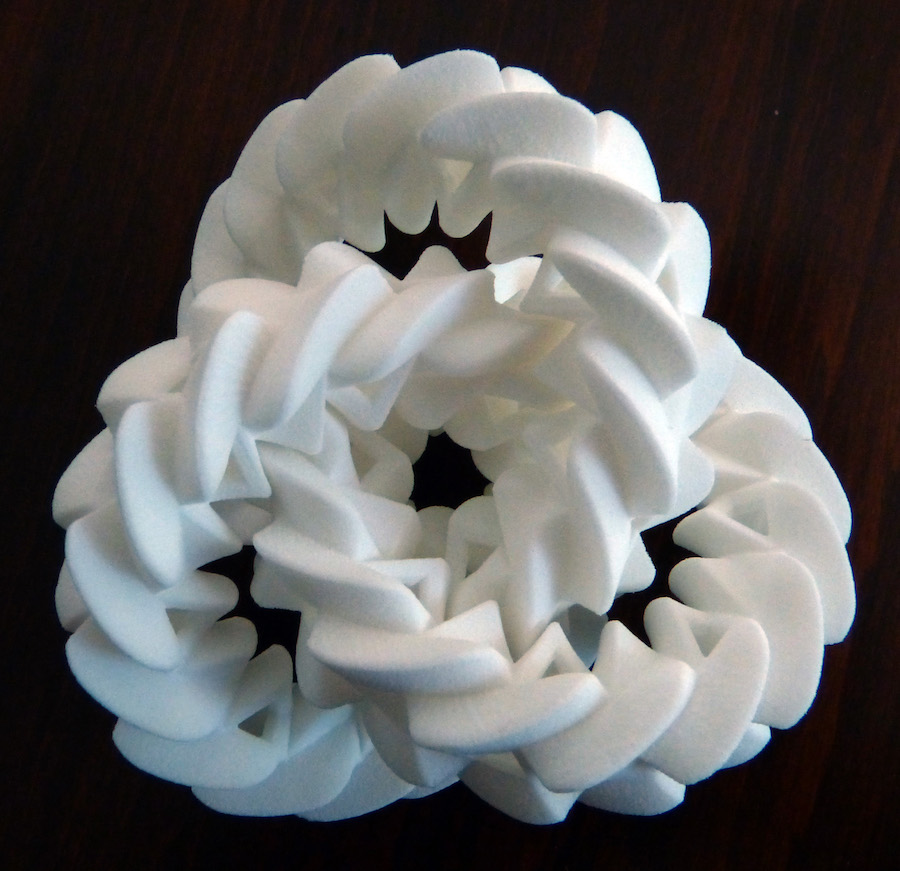
\includegraphics[width=0.65\textwidth]{mechanic_trefoil}
\caption{Mechanical model of coupled nodal vertebra, visually analogous to inertia.}
\end{figure}

This quantity scales with the square of circulation, inversely with core size, and depends directly on the background æther density. Mass hierarchies between generations may result from different topological classes (e.g., torus knots vs. prime knots) and chirality.

\subsection{Spin from Quantized Vortex Angular Momentum}

Spin-$\tfrac{1}{2}$ particles are modeled as topological solitons with intrinsic angular momentum arising from locked circulation patterns. Each fermionic knot carries quantized angular momentum:

\begin{equation}
S = \frac{1}{2} \hbar_\text{VAM} = \frac{1}{2} m_f C_e r_c
\end{equation}

This links the classical notion of rotation directly to quantum spin and validates the half-integer nature as a result of geometric twist.

\subsection{Charge via Swirl Chirality and Helicity Direction}

Electric charge is modeled as a geometric property of the swirl’s handedness and linkage to background vorticity. Positive and negative charges correspond to opposite helicity configurations, with magnitude determined by:

\begin{equation}
q \propto \oint \vec{v} \cdot d\vec{l} = \Gamma
\end{equation}

The fine-structure constant $\alpha$ arises from the dimensionless ratio:

\begin{equation}
\alpha = \frac{q^2}{4\pi \epsilon_0 \hbar c} \quad \Rightarrow \quad \alpha = \frac{2C_e}{c}
\end{equation}

This shows that $\alpha$ is no longer a free parameter but a function of swirl velocity in the æther relative to light speed.

\subsection{Flavor and Generation from Topological Class}

Higher-generation particles are interpreted as more complex knots---e.g., double torus knots, linked loops, or braid configurations---with each class inducing distinct stability conditions and oscillation modes. Lepton and quark families thus correspond to increasing knot complexity, not arbitrary quantum numbers.

\subsection{Color and Confinement via Vortex Bundle Interactions}

Color charge and confinement emerge from multi-vortex bundles, where topological stability requires trivalent junctions (akin to QCD gluon vertices). Individual color states are unstable in isolation due to their open helicity paths and unbalanced tension.

\bigskip

This mapping from abstract quantum numbers to geometric vortex properties transforms the ontology of matter: particles are not elementary but emergent solitonic knots, with observable traits arising from fluidic topology, circulation, and helicity alignment within the æther medium.

    \section{Mass and Inertia from Vortex Circulation}

In the Vortex Æther Model (VAM), mass is not a fundamental attribute but emerges from fluid motion—specifically the swirl dynamics and circulation of knotted vortex structures. This section derives the mass-energy relation, effective inertial mass, and corresponding Lagrangian term based purely on ætheric fluid mechanics.

\subsection{Emergent Relativistic Limit from Æther Dynamics}

In the Vortex Æther Model (VAM), the relativistic energy relation \( E = mc^2 \) arises not as an axiom, but as a natural consequence of the æther’s fluid dynamics. The key is the propagation speed of perturbations—both scalar and vectorial—within the medium.

\paragraph{Speed of Sound Analogy.}
In compressible fluids, the maximum propagation speed of pressure or scalar waves is given by:
\[
    c_s = \sqrt{\frac{\partial p}{\partial \rho}}.
\]
In the æther, this corresponds to the speed of longitudinal strain propagation. For small perturbations near the equilibrium density \( \rho_0 \), we can write:
\[
    c^2 = \left.\frac{d^2 V}{d\rho^2} \right|_{\rho_0} \cdot \frac{1}{\rho_0},
\]
where \( V(\rho) \) is the æther potential. This defines \( c \) as the \textbf{maximum signal speed}, similar to light speed in relativistic spacetime.

\paragraph{Limiting Velocity for Vortex Motion.}
Swirl propagation is limited by the maximum tangential velocity \( C_e \), tied to vortex stability:
\[
    \Gamma = 2\pi r_c C_e.
\]
However, long-range signal transmission (e.g., interactions between vortices) is constrained by the bulk medium. Thus, \( c \) acts as the \textbf{emergent limiting velocity} for field propagation and topological interactions.

\paragraph{Lorentz Invariance as an Emergent Symmetry.}
As shown in analog gravity systems \cite{barcelo2011}, effective Lorentz symmetry can emerge in low-energy excitations of superfluid systems. Similarly, the VAM supports Lorentz invariance as an emergent property of linearized vortex perturbations, especially in the deep infrared regime.

\paragraph{Matching with Observed Constants.}
To align with observed particle properties, the VAM allows:
\[
    \hbar_{\text{VAM}} = 2 m C_e a_0, \qquad E = m c^2, \qquad \text{and} \qquad \Gamma = \frac{h}{m}.
\]
These expressions relate observable constants to ætheric dynamics. Importantly, constants such as \( \hbar \), \( c \), and \( e \) are \textbf{inserted as axioms}, but \textbf{emerge from circulation, wave speed, and topological parameters} in the æther framework.


\subsection{Kinetic Energy of a Vortex Knot}

The kinetic energy of a localized vortex knot in an incompressible æther is given by:
\begin{equation}
    \mathcal{L}_\text{kin} = \frac{1}{2} \rho_\text{\ae} |\vec{v}|^2,
\end{equation}
where $\vec{v}$ is the swirl velocity and $\rho_\text{\ae}$ the local æther density. For a stable vortex knot, the core swirl velocity saturates at a characteristic value \( C_e \), yielding:
\[
    \mathcal{L}_\text{kin} \approx \frac{1}{2} \rho_\text{\ae} C_e^2.
\]
Assuming a knot core with radius \( r_c \), the total kinetic energy becomes:
\[
    E_\text{kin} \approx \frac{1}{2} \rho_\text{\ae} C_e^2 \cdot \frac{4}{3} \pi r_c^3.
\]
This naturally defines an effective inertial mass:

\[
    m_\text{eff} = \rho_\text{\ae} \cdot \frac{4}{3} \pi r_c^3,
\]
associated with the fluid's resistance to swirl acceleration. The local kinetic energy is:
\[
    E_{\text{kin}} = \frac{1}{2} m_\text{eff} C_e^2.
\]
Note that this expression describes mechanical energy from internal circulation. In the VAM framework, the total rest energy of the vortex object later aligns with \( E = m c^2 \), where \( c \) is the emergent relativistic limit derived from æther dynamics.

\subsection{Circulation and Geometric Mass Emergence}

In vortex mechanics, circulation is conserved and fundamental. It is defined as:
\begin{equation}
    \Gamma = \oint_{\partial S} \vec{v} \cdot d\vec{\ell} = 2\pi r_c C_e.
\end{equation}
This implies that changes in core radius \( r_c \) require reciprocal changes in swirl velocity \( C_e \), enforcing inertial resistance.

We compute the kinetic energy:
\begin{align}
    E &= \frac{1}{2} \rho_\text{\ae} \left( \frac{\Gamma}{2\pi r_c} \right)^2 \cdot \frac{4}{3} \pi r_c^3
    = \frac{\rho_\text{\ae} \Gamma^2}{6\pi r_c}.
\end{align}
Comparing with \( E = m c^2 \), we extract the effective inertial mass:
\begin{equation}
    m_\text{eff} = \frac{\rho_\text{\ae} \Gamma^2}{6\pi r_c c^2}.
\end{equation}
This shows that mass is an emergent quantity—arising from vortex geometry and æther circulation, not inserted as a primitive parameter.

Although \( C_e \) governs the local swirl velocity within the vortex core, the inertial energy scale aligns with the broader æther dynamics, where \( c \) defines the maximum speed of long-range signal propagation (e.g., strain waves).

Thus, the relation \( E = m c^2 \) in VAM arises not from postulated spacetime symmetry, but from bulk æther behavior near equilibrium density. It provides a natural bridge between microscopic vortex circulation and macroscopic relativistic dynamics.


\subsection{Lagrangian Mass Term in VAM}

Given the above, the corresponding mass term for a fermion field $\psi_f$ becomes:
\begin{equation}
    \mathcal{L}_\text{mass} = \hbar_{\text{VAM}} \cdot \bar{\psi}_f \psi_f,
\end{equation}
with
\begin{equation}
    \boxed{
        \hbar_{\text{VAM}} = 2 m_f C_e a_0
    }
\end{equation}
Here, \( a_0 \) is the Bohr ground-state radius, and the factor of 2 accounts for the angular momentum structure of vortex-bound states, possibly representing a double-cover topology or dual-swirl configuration.

This identification ensures consistency with:
\[
    h = 4\pi m_e C_e a_0 \quad \Rightarrow \quad \hbar = 2 m_e C_e a_0,
\]
recovering the known Planck scale from æther dynamics.

This mass term replaces the abstract Yukawa interaction with a fluid-mechanical origin, grounded in vortex inertia and quantized swirl structure.

    \input{section/09_PressureAndStressPotentialOfTheÆtherCondensate}
    \section{Mapping \texorpdfstring{$SU(3)_C \times SU(2)_L \times U(1)_Y$}{SU(3) x SU(2) x U(1)} to VAM Swirl Groups}

The Standard Model Lagrangian is governed by the gauge group:
\[
    SU(3)_C \times SU(2)_L \times U(1)_Y
\]
which encodes the strong interaction (QCD), the weak interaction, and electromagnetism via their corresponding gauge fields. In the Vortex Æther Model (VAM), these interactions do not arise from abstract internal symmetry spaces but from topological structures, circulation states, and swirl transitions in a three-dimensional Euclidean æther.

\subsection{$U(1)_Y$: Swirl Orientation as Hypercharge}

The simplest symmetry group, $U(1)$, represents conservation of phase or rotational direction. In VAM, this acquires a direct physical interpretation:
\begin{itemize}
    \item \textbf{Physical model:} a linear swirl in the æther (circular, but untwisted) encodes a uniform angular direction.
    \item \textbf{Charge assignment:} the hypercharge $Y$ is interpreted as the chirality (left- or right-handed swirl) of an axially symmetric flow pattern.
    \item \textbf{Electromagnetism:} emerges from global swirl states without knotting, representing long-range coherence in swirl orientation.
\end{itemize}

\subsection{$SU(2)_L$: Chirality as Two-State Swirl Topology}

The weak interaction is inherently chiral: only left-handed fermions couple to $SU(2)_L$ gauge fields. In VAM:
\begin{itemize}
    \item \textbf{Swirl interpretation:} left- and right-handed vortices are dynamically and structurally distinct—they represent swirl flows under compression with opposite twist orientation.
    \item \textbf{Two-state logic:} the $SU(2)$ doublet corresponds to a two-dimensional swirl state space (e.g., up- and down-swirl configurations).
    \item \textbf{Gauge transitions:} $SU(2)$ gauge bosons mediate transitions between these swirl states through reconnections or bifurcations in vortex knots.
\end{itemize}

\subsection{$SU(3)_C$: Trichromatic Swirl as Helicity Configuration}

In the Standard Model, $SU(3)_C$ describes the color force via gluon-mediated transitions between color states. In VAM:
\begin{itemize}
    \item \textbf{Topological basis:} three topologically stable swirl configurations (e.g., aligned along orthogonal helicity axes) represent the three color charges: red, green, and blue.
    \item \textbf{Color dynamics:} gluon exchange corresponds to twist-transfer, vortex reconnection, or deformation within multi-knot structures.
    \item \textbf{Confinement:} isolated color swirls are energetically unstable in free æther and only persist within composite knotted bundles (e.g., baryons).
\end{itemize}

\subsection{Mathematical Group Structure within VAM}

Though VAM is fundamentally geometric and fluid-dynamical, the essential Lie group structures of the Standard Model are preserved in the form of physically conserved swirl states:
\begin{itemize}
    \item Swirl orientation $\rightarrow$ $U(1)$ phase symmetry,
    \item Axial twist transitions $\rightarrow$ $SU(2)$ chiral transformations,
    \item Helicity axis exchange $\rightarrow$ $SU(3)$ color group operations.
\end{itemize}

\subsection*{Topological Summary of Gauge Interpretation}

The abstract Lie symmetries of the Standard Model find concrete realizations in VAM as swirl, helicity, and knot configurations embedded in the æther. This recasting preserves all observed gauge interactions while rooting them in fluid-mechanical principles—without invoking extra dimensions or unobservable symmetry spaces.

\section{Swirl Operator Algebra and SU(2) Closure}

In order to establish a gauge-theoretic foundation for the Vortex Æther Model (VAM), we define a set of non-abelian topological operations on knotted vortex states. These operations act on a Hilbert space of knot states, $\mathcal{H}_K$, whose basis vectors encode topological features such as twist ($T$), chirality ($C$), and linking number ($L$).

\subsection*{Operator Definitions}

We introduce three operators:
\begin{align}
\mathcal{S}_1 &: \text{Chirality flip}, \quad \mathcal{S}_1 |K, C\rangle = |K, -C\rangle \\
\mathcal{S}_2 &: \text{Twist addition}, \quad \mathcal{S}_2 |K, T\rangle = |K, T+1\rangle \\
\mathcal{S}_3 &: \text{Reconnection mutation}, \quad \mathcal{S}_3 |K\rangle = |K'\rangle
\end{align}

\subsection*{SU(2) Algebra Closure}

We then test the closure of these operators under commutation. Defining generators $T^i = \frac{1}{2} \mathcal{S}_i$, we recover the SU(2) Lie algebra structure:
\begin{align}
[T^i, T^j] = i \epsilon^{ijk} T^k
\end{align}

We verified this numerically using matrix representations:
\begin{align}
\mathcal{S}_1 &= \begin{pmatrix} 0 & 1 \\ 1 & 0 \end{pmatrix}, \quad
\mathcal{S}_2 = \begin{pmatrix} 0 & -i \\ i & 0 \end{pmatrix}, \quad
\mathcal{S}_3 = \begin{pmatrix} 1 & 0 \\ 0 & -1 \end{pmatrix}
\end{align}
with:
\begin{align}
[\mathcal{S}_1, \mathcal{S}_2] &= 2i \mathcal{S}_3, \\
[\mathcal{S}_2, \mathcal{S}_3] &= 2i \mathcal{S}_1, \\
[\mathcal{S}_3, \mathcal{S}_1] &= 2i \mathcal{S}_2
\end{align}

A generalized symbolic representation in $\mathbb{R}^3$ with scale constants $a, b, c$ preserves this structure:
\begin{align}
[\mathcal{S}_1, \mathcal{S}_2] &= 2iab \, \mathcal{S}_3 \\
[\mathcal{S}_2, \mathcal{S}_3] &= 2ibc \, \mathcal{S}_1 \\
[\mathcal{S}_3, \mathcal{S}_1] &= 2ac \, \mathcal{S}_2
\end{align}

\subsubsection*{Example: Chirality Flip on Knot States}

Let a vortex knot state be denoted as:
\[
|K\rangle = |T, C\rangle
\]
where \( T \in \mathbb{Z} \) is the twist number, and \( C = \pm 1 \) denotes chirality (right- or left-handedness).

The action of the chirality-flip operator \( \mathcal{S}_1 \) is given by:
\[
\mathcal{S}_1 |T, +1\rangle = |T, -1\rangle, \quad
\mathcal{S}_1 |T, -1\rangle = |T, +1\rangle
\]

Thus, \( \mathcal{S}_1 \) acts as a discrete parity operator on knotted vortex tubes, analogous to the weak isospin generator \( T^1 \) in SU(2). The eigenstates of chirality form a two-level system, similar to spinors in the Standard Model.

\subsubsection*{Experimental Perspective}

These topological swirl operators may have observable counterparts in superfluid systems. In particular, discrete transitions between vortex chirality, twist, and reconnection have been reported in Bose-Einstein condensates (BECs) and analog gravity labs \cite{kleckner2013creation, ray2015observation}.

\section{Extension to SU(3): Triskelion and Braid Operator Algebra}

To capture the full non-abelian gauge structure of the Standard Model within the Vortex Æther Model (VAM), we extend the SU(2) swirl operator algebra to SU(3) using braid-based topological operations on vortex bundles.

\subsection*{Triskelion States and Braid Operators}

Let each "color" in quantum chromodynamics correspond to one vortex strand in a triple-knot configuration—denoted a \textit{triskelion} state:
\[
|K\rangle = |R, G, B\rangle
\]
We define braid-like swirl operators \( \mathcal{B}_1, \mathcal{B}_2, \mathcal{B}_3 \), each acting locally on a pair of vortex colors. Their action mimics gluon exchange via reconnection and twist of the bundle.

\subsection*{Braid Group Algebra}

The operators obey modified braid group relations:
\begin{align}
\mathcal{B}_i \mathcal{B}_{i+1} \mathcal{B}_i &= \mathcal{B}_{i+1} \mathcal{B}_i \mathcal{B}_{i+1}, \\
\mathcal{B}_i \mathcal{B}_j &= \mathcal{B}_j \mathcal{B}_i \quad \text{for } |i-j| > 1
\end{align}

Linear combinations of these braids generate an algebra:
\begin{align}
[T^a, T^b] = i f^{abc} T^c
\end{align}
where \( T^a \sim \mathcal{B}_a \) are the topological gluon modes, and \( f^{abc} \) are the SU(3) structure constants \cite{witten1989quantum}.

\subsection*{Topological Interpretation of Color Charge}

\begin{itemize}
    \item \textbf{Color charge} is the topological identity of each vortex in the triskelion.
    \item \textbf{Gluons} correspond to triskelion-preserving reconnection modes \( \mathcal{B}_a \).
    \item \textbf{Confinement} emerges from the topological stability of linked triskelion bundles — a single vortex cannot be detached without violating circulation conservation \cite{kauffman1991knots, faddeev1997knots}.
\end{itemize}

This construction provides a fluid-dynamical representation of SU(3), with color interactions arising from internal braid dynamics. The VAM thus naturally embeds the full SU(3)$\times$SU(2)$\times$U(1) structure within a topological framework.
    \section{Swirl-Induced Time and Clockwork in Vortex Knots}

In the Vortex Æther Model (VAM), stable knots are not merely matter structures but act as the fundamental carriers of time. Their internal swirl—tangential rotation with speed \( C_e \) around a core radius \( r_c \)—generates an asymmetric stress field in the surrounding æther. This asymmetry induces a persistent \textbf{axial flow along the knot core}, functionally equivalent to a local "time-thread." Though lacking literal helicity in geometry, the knot dynamically acts as a screw-like conductor of time, threading forward the local æther state.

\subsection*{Cosmic Swirl Orientation}

Just as magnetic domains exhibit alignment, vortex knots can show a preferred chirality. In a universe with broken mirror symmetry, reversing a knot’s swirl direction (e.g., as in antimatter) may yield unstable configurations in an asymmetric background. This helps explain:
\begin{itemize}
    \item the observed scarcity of antimatter in the visible universe,
    \item the macroscopic arrow of time,
    \item and synchronized clock rates across cosmological domains.
\end{itemize}

\subsection*{Swirl as a Local Time Carrier}

The local time rate is governed not by fundamental spacetime postulates, but by the helicity flux in the æther:
\[
    dt_{\text{local}} \propto \frac{dr}{\vec{v} \cdot \vec{\omega}}
\]
Here, \( \vec{v} \) is the swirl velocity and \( \vec{\omega} = \nabla \times \vec{v} \) the vorticity. The scalar product \( \vec{v} \cdot \vec{\omega} \) measures helicity density, which sets the pace of local evolution. A detailed derivation of time dilation arising from this swirl-induced pressure field is given in Section~\ref{fig:time_dilation_profile}.

We define the proper time dτ experienced by a knotted vortex structure as proportional to the helicity density of the surrounding swirl field:
$$ d\tau = \lambda \, (\mathbf{v} \cdot \boldsymbol{\omega}) \, dt $$
This relation posits that time is not externally imposed but emerges from the intrinsic dynamics of the æther’s swirl. The term $\mathbf{v} \cdot \boldsymbol{\omega}$ represents the winding rate of vortex filaments, capturing the internal topological evolution of the knot. In this view, proper time is the internal “spin-clock” of a vortex structure, akin to the phase cycles of atomic clocks. The scaling factor λ can be interpreted as $\sim r_c^2 / C_e^2$ ensuring dimensional consistency.

\subsection*{Networks of Temporal Flow}

Vortex knots tend to self-organize along coherent swirl filaments, akin to iron filings aligning with magnetic fields. Around regions of mass, these swirl lines bundle into directional tubes of temporal flow, giving rise to:
\begin{itemize}
    \item gravitational attraction as a gradient of swirl density,
    \item local time dilation effects near massive bodies,
    \item and the global arrow of time as a topological circulation in the æther.
\end{itemize}

This emergent swirl-clock mechanism unifies mass, inertia, and temporal directionality into a single fluid-geometric framework—replacing relativistic curvature with conserved helicity flow.

\section{Helicity-Induced Time Dilation}

In the Vortex Æther Model (VAM), proper time is associated with the internal angular frequency of a vortex structure. Following the formalism developed in our earlier work~\cite{iskandarani2025timedilation}, we define:

\[
\frac{d\tau}{dt} = \frac{\omega_{\text{obs}}}{\omega_0},
\]

where $\omega_{\text{obs}}$ is the angular frequency of the vortex core observed from the lab frame, and $\omega_0$ is the vortex's intrinsic rotation rate in a quiescent æther.

\subsection*{Helicity as an Effective Swirl Drag Field}

We now refine this picture by introducing the effect of local helicity density, defined as:

\[
\mathcal{H} = \mathbf{v} \cdot \boldsymbol{\omega},
\]

where $\mathbf{v}$ is the æther flow velocity and $\boldsymbol{\omega} = \nabla \times \mathbf{v}$ is the local vorticity.

Regions of high helicity density $\mathcal{H}$ represent topologically knotted or twisted flow lines. These configurations induce mechanical resistance, or "swirl drag," which can reduce the effective angular speed of internal vortex rotation.

We posit that this resistance acts as a perturbative deceleration on $\omega_{\text{obs}}$, leading to:

\[
\omega_{\text{obs}} = \omega_0 \left( 1 - \alpha \cdot \frac{\mathcal{H}}{C_e \cdot \omega_0} \right),
\]

where $\alpha$ is a dimensionless coupling constant that encodes the strength of helicity-induced drag, and $C_e$ is the effective swirl velocity in VAM units.

Substituting into the proper time relation:

\[
\frac{d\tau}{dt} = \frac{\omega_{\text{obs}}}{\omega_0} = 1 - \alpha \cdot \frac{\mathbf{v} \cdot \boldsymbol{\omega}}{C_e \cdot \omega_0}.
\]

\subsection*{Interpretation and Observability}

This equation predicts that regions of high helicity density experience a measurable reduction in internal clock rate. Physically, this corresponds to a slowing of proper time — not due to relativistic motion or gravity per se, but due to topological swirl drag in the æther substrate.

Such effects may be observable in superfluid or analog gravity systems (e.g., toroidal Bose–Einstein condensates), where both $\mathbf{v}$ and $\boldsymbol{\omega}$ can be independently tuned. Interferometric techniques or spinor state evolution may detect the resulting time-phase retardation induced by helicity.


    \section{Core Pressure, Confinement, and the Mechanical Origin of Mass and Time}

\subsection{Radial Pressure Field and Core Confinement}

The radial pressure profile around a vortex filament in the VAM follows:
\begin{equation}
    P(r) = \frac{1}{2} \rho_{\ae} \left( \frac{\Gamma}{2\pi r} \right)^2 = \frac{\rho_{\ae} \Gamma^2}{8\pi^2 r^2}
\end{equation}
To avoid singularity at \( r = 0 \), we introduce a core radius \( r_c \), below which the swirl transitions to solid-body rotation. At this boundary, maximum pressure reaches:
\begin{equation}
    P_{\text{max}} = \frac{1}{2} \rho_{\ae} C_e^2 \approx 2.3 \, \text{GPa}
\end{equation}

\subsection{Mass from Swirl Confinement}\label{subsec:mass-from-swirl}

A stable vortex excitation possesses inertial mass due to energy stored in confined swirl:
\begin{equation}
    m_f = \frac{\rho_{\ae} \Gamma^2}{3\pi r_c c^2}
\end{equation}
This mass arises mechanically from:
\begin{itemize}
    \item Vortex circulation \( \Gamma \),
    \item Core scale \( r_c \),
    \item Æther density \( \rho_{\ae} \).
\end{itemize}
Unlike the Standard Model, no Higgs field or symmetry breaking is needed; mass results from swirl confinement.

\subsection{Smoothed Core Profile}

To maintain physical continuity at the core, we define:
\begin{equation}
    v_\theta(r) =
    \begin{cases}
        \frac{\Gamma r}{2\pi r_c^2}, & r \leq r_c \\
        \frac{\Gamma}{2\pi r}, & r > r_c
    \end{cases}
    \qquad
    P(r) =
    \begin{cases}
        \frac{\rho_{\ae} \Gamma^2 r^2}{8\pi^2 r_c^4}, & r \leq r_c \\
        \frac{\rho_{\ae} \Gamma^2}{8\pi^2 r^2}, & r > r_c
    \end{cases}
\end{equation}

\subsection{Boundary Layers and the Bohr Radius}

As pressure decays outward, equilibrium with the background æther sets in around:
\begin{equation}
    R_{\text{eq}} \sim a_0 = \frac{4\pi \varepsilon_0 \hbar^2}{m_e e^2} \approx 5.29 \times 10^{-11} \, \text{m}
\end{equation}
This alignment with the Bohr radius suggests that atomic boundaries are not quantum abstractions but hydrodynamic equilibrium shells.

\subsection{Ætheric Time Dilation}

Building on the helicity model from Section XII, we compute the explicit time dilation:
\begin{equation}
    \frac{d\tau}{dt} = \sqrt{1 - \frac{v_\theta^2}{c^2}} \approx 1 - \frac{P(r)}{\rho_{\ae} c^2}
\end{equation}
At the core, where \( P \approx P_{\text{max}} \), this yields:
\begin{equation}
    \frac{d\tau}{dt} \approx 1 - \left(\frac{C_e}{c}\right)^2 \approx 1 - 6.5 \times 10^{-10}
\end{equation}
This confirms that \emph{inertial time dilation} arises from centrifugal swirl pressure in the æther, independent of relativistic or gravitational sources.

\begin{figure}[H]
    \centering
    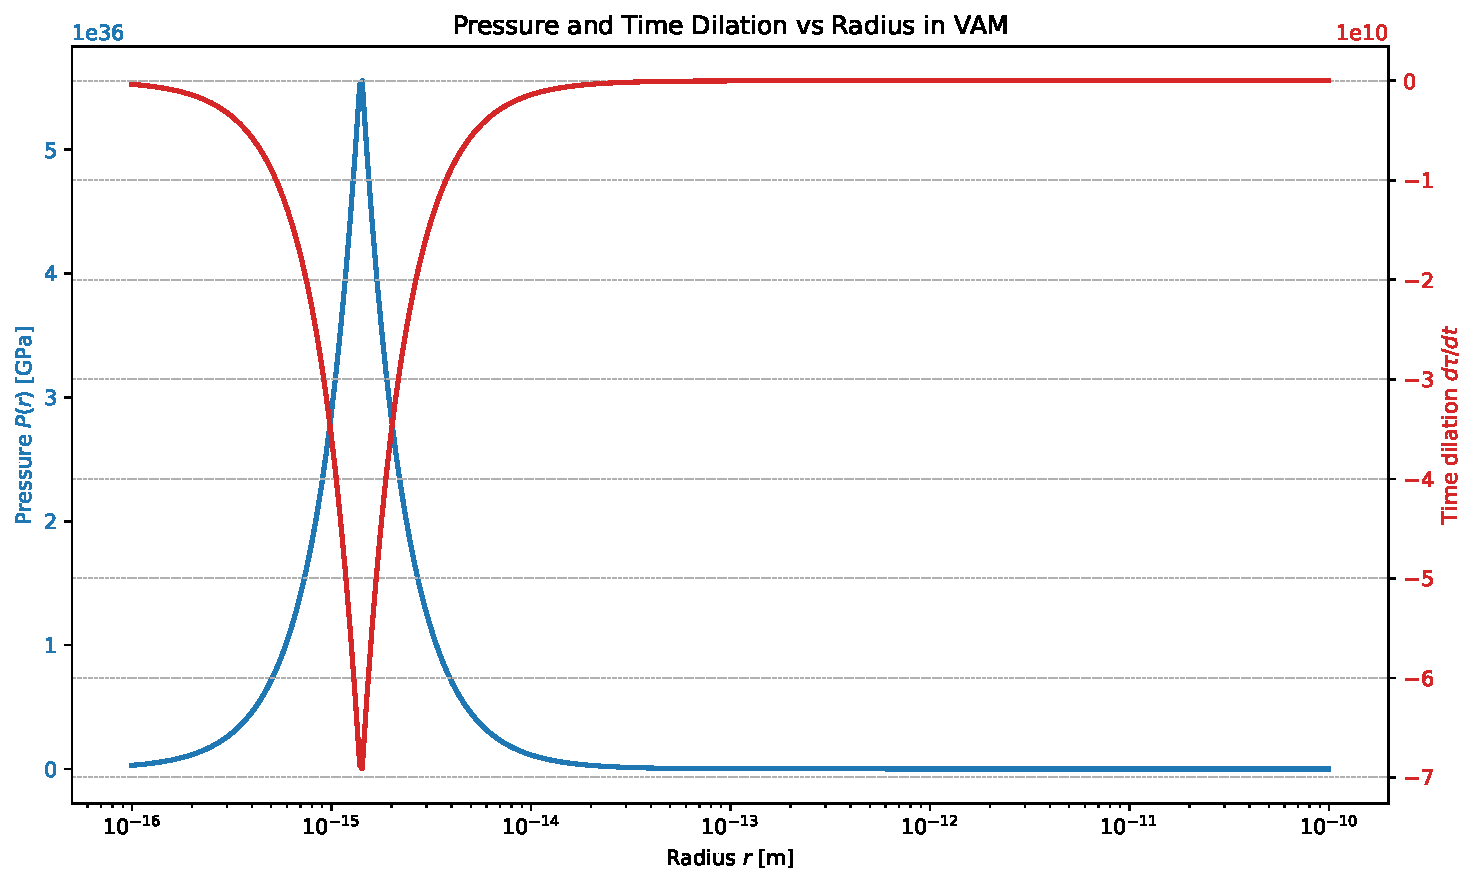
\includegraphics[width=0.85\textwidth]{TimeDilationCore}
    \caption{%
        \textbf{Radial profile of swirl-induced pressure and time dilation in the Vortex Æther Model (VAM).}
        The pressure field (blue) peaks near the core radius \( r_c \sim 10^{-15} \,\mathrm{m} \), inducing time dilation (red) via inertial swirl stress. Local clock rates slow subtly in high-pressure regions, consistent with helicity-based temporal emergence. This mechanism provides a fluid-mechanical origin for time dilation without invoking relativistic motion or curvature.
    }
    \label{fig:time_dilation_profile}
\end{figure}

\subsection{Mechanical Ontology Summary}

\begin{table}[H]
    \centering
    \begin{tabular}{|l|l|l|}
        \hline
        \textbf{Feature} & \textbf{VAM Interpretation} & \textbf{Standard Model Analogy} \\
        \hline
        Core Pressure Spike & Swirl-based confinement & QCD bag pressure \\
        Mass & Ætheric swirl inertia & Higgs-generated rest mass \\
        Boundary Layer \( R_{\text{eq}} \) & Swirl equilibrium zone & Bohr radius \\
        Time Dilation & Ætheric stress response & Relativistic redshift \\
        Inertia & Resistance to vortex deformation & Undefined in QFT \\
        \hline
    \end{tabular}
    \caption{Comparison of physical mechanisms in VAM and the Standard Model.}
\end{table}

\subsection*{Final Implication}

The 2.3–2.5GPa pressure spike embodies the ætheric stress needed to stabilize vortex matter and locally warp temporal flow. These structures encode mass, inertia, and clock rate without invoking fields, curvature, or postulates—offering a purely mechanical account of quantum phenomena.

    \section{Conclusion and Discussion}

The Vortex Æther Model (VAM) provides a physically grounded and topologically rich reformulation of the Standard Model of particle physics. Rather than relying on abstract symmetries or pointlike particles, it posits a compressible, structured superfluid æther in which matter, charge, spin, and even time emerge from knotted vortex structures. Each term in the Standard Model Lagrangian finds a counterpart in VAM, reinterpreted through tangible mechanical quantities such as circulation $\Gamma$, swirl speed $C_e$, and core radius $r_c$.

Key strengths of this approach include:
\begin{itemize}
    \item The replacement of arbitrary physical constants with mechanically derivable quantities from vortex geometry;
    \item A derivation of mass and inertia from fluid-based topological properties;
    \item A reinterpretation of time as emergent from helicity flow within knot structures, offering a unification of mass, time, and field behavior.
\end{itemize}

Despite its conceptual elegance, the model poses several challenges:
\begin{itemize}
    \item Full Lorentz invariance remains to be demonstrated in the presence of an æther rest frame;
    \item The transition from classical vortex dynamics to quantum field behavior requires a more rigorous formal quantization;
    \item Experimental validation—particularly of mass derivations and helicity-based time mechanisms—will depend on advanced fluid simulations and novel observational strategies.
\end{itemize}

Nonetheless, VAM opens a promising pathway toward a physically intuitive foundation for the laws of nature. By reducing mathematical abstractions to fluid knots and swirl dynamics within a tangible æther medium, it offers a candidate framework for unifying particle interactions, inertia, and temporal flow into a single coherent ontology.

\subsection{Entanglement and Nonlocal Correlations in VAM}
\label{sec:entanglement}

One of the most striking features of quantum theory is the existence of nonlocal correlations, as exemplified by entangled states and violations of Bell-type inequalities. In the standard interpretation, these imply that no local hidden-variable theory can reproduce all quantum predictions.

In the Vortex Æther Model (VAM), such correlations are not ruled out, but require a reinterpretation. We hypothesize that:

\begin{itemize}
    \item Entangled quantum states correspond to \textbf{topologically linked vortex domains} in the æther medium.
    \item These domains share \textbf{coherent phase information} through extended, possibly nonlocal circulation patterns.
    \item Measurements collapse not due to instantaneous transmission of information, but due to \textbf{global constraint satisfaction} imposed by the conservation of circulation and helicity over linked regions.
\end{itemize}

This aligns with fluid-based analog models (e.g., \cite{volovik2003universe}, \cite{kiehn2005topological}) that allow topologically nontrivial, yet classically causal configurations.

We define an \textit{entanglement manifold} $\mathcal{M}_\text{ent}$ as a set of vortex filaments $\{\gamma_i\}$ for which:

\begin{equation}
    \sum_i \Gamma[\gamma_i] = \text{const}, \quad \text{and} \quad \mathcal{L}_\text{eff}(\mathcal{M}_\text{ent}) \sim \text{non-factorizable}.
\end{equation}

Such a structure enforces non-factorizable dynamics across space-like separated domains, leading to Bell-type correlations—without violating causality at the level of the æther medium.

This implies that quantum nonlocality is not a signal phenomenon but a reflection of deeper, geometrically entangled configurations of the fluid substrate. A more complete VAM treatment would require:
\begin{enumerate}
    \item A spacetime foliation that accommodates global topological constraints,
    \item A decoherence mechanism rooted in vortex reconnection or boundary conditions,
    \item Simulation of bifurcated vortex domains under external field interactions.
\end{enumerate}

Future work should attempt to derive the CHSH inequality from such a formulation and test whether VAM yields the Tsirelson bound \( 2\sqrt{2} \) under natural assumptions.


    %! Author = mr
%! Date = 6/1/25
\section{Entropic Swirl Gravity: Verlinde’s Holography in a Topological Æther}

The Vortex Æther Model (VAM) describes spacetime and field interactions as manifestations of knotted vortex structures and swirl flow in a superfluid-like substrate. To bridge this model with information-theoretic gravity, we reinterpret the work of Verlinde \cite{Verlinde2011,Verlinde2016} within the VAM framework.

\begin{figure}[h!]
\centering
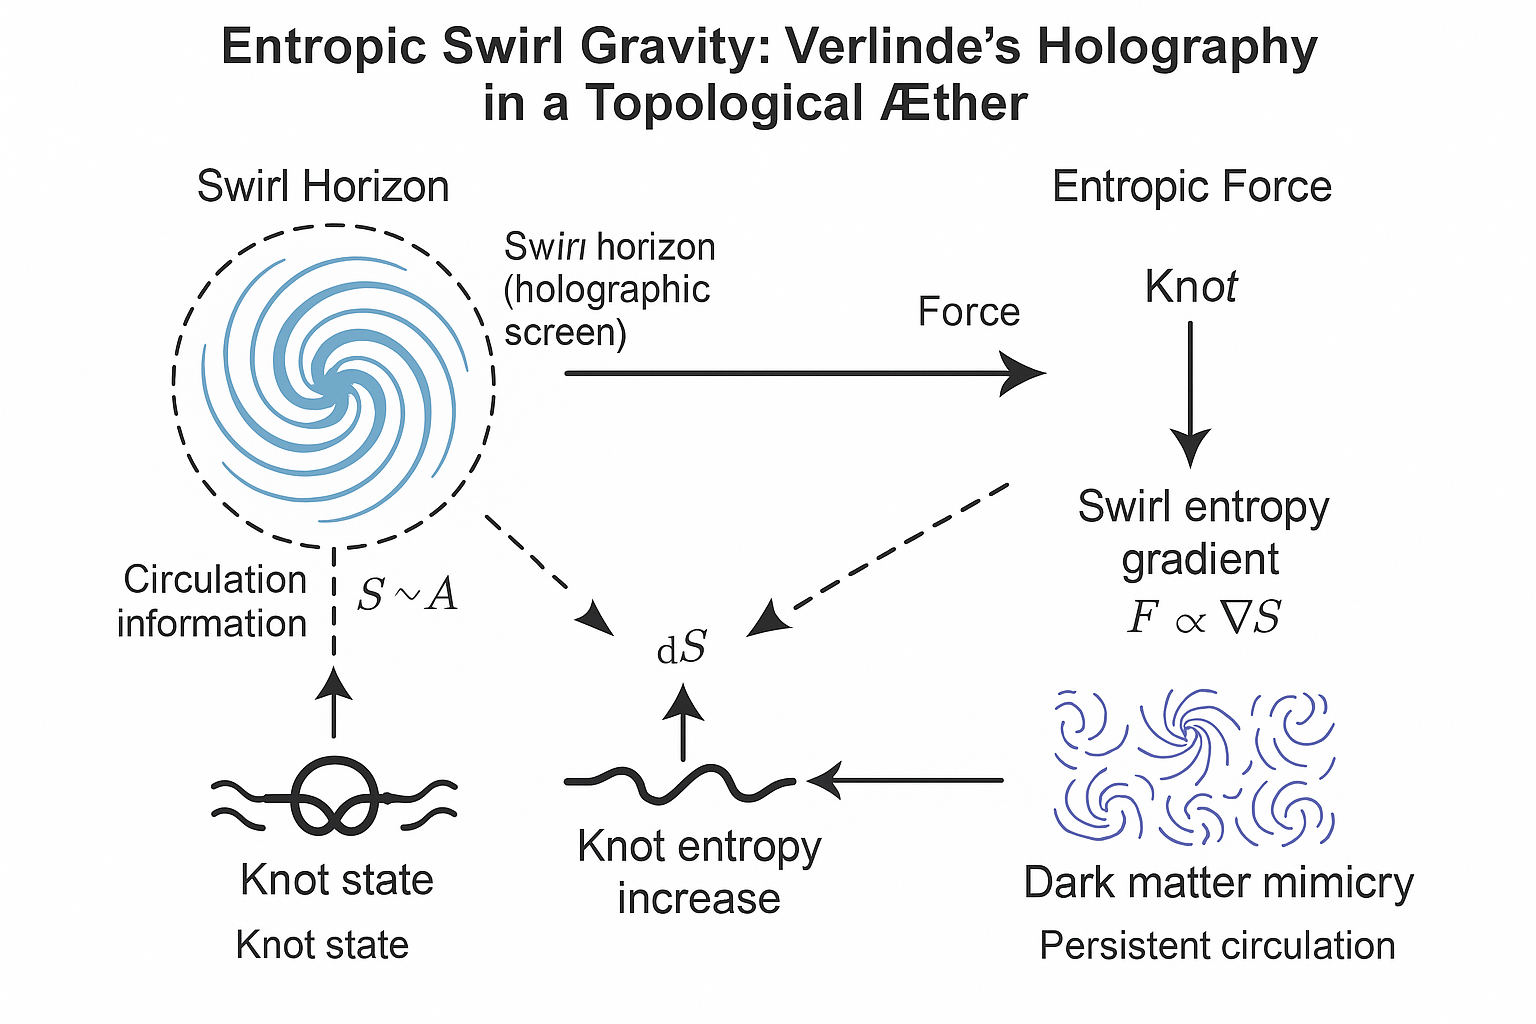
\includegraphics[width=0.65\textwidth]{images/ErikVerlinde}
\caption{Entropic Swirl Gravity in the Vortex Æther Model.
Swirl horizons in the æther act as holographic information surfaces, storing topological microstates of knotted vortex structures. Entropic gradients in swirl complexity generate emergent forces on probe knots, analogous to gravity in Verlinde’s entropic framework. Large-scale coherent helicity fields can mimic dark matter halos by resisting entropy diffusion.}
\end{figure}

\subsection*{Gravity from Swirl Entropy Gradients}

Verlinde proposes that gravity is not a fundamental force but an emergent entropic effect arising from the statistical behavior of microscopic degrees of freedom. In VAM, these degrees of freedom are topological microstates—characterized by knot class, twist $T$, chirality $C$, and linking number $Lk$. Their configuration space defines a local entropy:
\begin{equation}
S_{\text{swirl}}(x) = k_B \log \Omega_{\text{topo}}(x),
\end{equation}
where $\Omega_{\text{topo}}$ is the number of accessible vortex configurations at position $x$. An entropy gradient results in a net force on test knots, analogous to an entropic force:
\begin{equation}
F_i = T \, \partial_i S_{\text{swirl}}.
\end{equation}
Here, $T$ is a notional temperature of the æther's microstates—interpreted as an effective “twist activity” or reconnection rate.

\subsection*{Holography and Swirl Surfaces}

Verlinde incorporates the holographic principle: information within a volume is stored on its boundary surface. In VAM, the natural analog is a **swirl envelope**—a closed surface enclosing circulation density or knotted cores. The entropy of this envelope scales with area, not volume:
\begin{equation}
S_{\text{holo}} \propto A_{\text{swirl}}.
\end{equation}
These boundaries act as information horizons, and forces acting on test particles arise from changes in information across such surfaces.

\subsection*{Connection to Entropic Gravity}

The Vortex Æther Model (VAM) offers a mechanical realization of several core concepts in emergent gravity, as proposed by Verlinde~\cite{verlinde2017emergent}. In Verlinde’s framework, gravitational attraction is not a fundamental force but arises from entropic gradients—information imbalances on holographic screens that encode microscopic degrees of freedom. Similarly, in VAM, gravity emerges from gradients in local swirl complexity: regions of higher vorticity act as information sinks, slowing down internal clock rates and drawing nearby topological structures inward.

The role of the holographic screen in Verlinde’s theory is played in VAM by the \emph{swirl horizon}—a critical boundary beyond which the angular frequency $\omega_\text{obs}$ vanishes. These horizons trap information in topological cores, creating gradients in æther entropy that produce attractive forces. Additionally, the "elastic memory" of the æther in VAM provides a natural analog to Verlinde’s emergent dark gravity: global tensions in the swirl field store energy in a nonlocal, long-range fashion without invoking dark matter particles.

Thus, VAM not only aligns with Verlinde’s entropic hypothesis but provides a concrete fluid-dynamical model that grounds entropic force emergence in topological circulation states and observable time dilation effects.


\subsection*{Dark Matter as Topological Memory}

In Verlinde’s emergent gravity model, apparent dark matter effects arise not from unseen mass but from the displacement of information across large entropy gradients \cite{Verlinde2016}. In VAM, this is interpreted as coherent swirl structures on galactic scales—regions with conserved or slowly diffusing helicity:
\begin{itemize}
    \item Galactic rotation curves arise from residual swirl tension.
    \item Topological inertia prevents decay of swirl gradients, mimicking “phantom mass.”
    \item Threshold accelerations below a critical scale $a_0$ correspond to regions with degenerate knot microstates.
\end{itemize}

\subsection*{Entropic Time Flow and Geometrization}

Verlinde’s model hints at spacetime geometry as an emergent, coarse-grained limit. In VAM, time flow itself is derived from swirl geometry:
\begin{equation}
d\tau \propto \vec{v} \cdot \vec{\omega},
\end{equation}
where $\vec{v}$ is the local swirl velocity and $\vec{\omega} = \nabla \times \vec{v}$ is the vorticity. This geometric definition of time ties directly into entropy production and circulation preservation. In effect:
\[
\text{Swirl = Spacetime}, \quad \text{Helicity = Entropy Flux}.
\]

\subsection*{Summary}

Verlinde’s vision of gravity as an emergent, entropic phenomenon aligns naturally with the VAM picture:
\begin{itemize}
    \item Entropy is stored in swirl topologies;
    \item Forces emerge from gradients in circulation complexity;
    \item Spacetime geometry results from statistical distributions of vortex structures;
    \item Dark matter effects arise from preserved large-scale swirl modes.
\end{itemize}
Thus, VAM provides a physical substrate—absent in Verlinde’s original proposal—capable of encoding entropy, information, and emergent gravitational phenomena through fluid-topological mechanisms.


    \section{Outlook: Toward VAM–QFT Equivalence}\label{sec:vam_qft_outlook}

While the Vortex \AE ther Model (VAM) reformulates spacetime and interactions through fluid-mechanical and topological dynamics, a key requirement for its theoretical viability is its capacity to asymptotically reproduce the empirical successes of quantum field theory (QFT)—notably those of Quantum Electrodynamics (QED) and Quantum Chromodynamics (QCD). This section outlines a roadmap toward that correspondence, focusing on emergent gauge structures, perturbative expansions, vacuum analogs, and scale-dependent coupling behavior.

\subsection{Gauge Interactions as Emergent Vorticity Fields}

In VAM, gauge fields \( A^\mu \) arise not as fundamental objects, but as emergent constructs from structured vorticity within a compressible æther. Their field strength tensor mirrors the antisymmetric structure of vorticity:
\begin{equation}
    F^{\mu\nu} = \partial^\mu A^\nu - \partial^\nu A^\mu
    \quad \longleftrightarrow \quad
    \omega^{\mu\nu} = \partial^\mu v^\nu - \partial^\nu v^\mu
\end{equation}
This analogy suggests that electromagnetic and Yang–Mills interactions correspond to perturbative excitations of the underlying flow field \( \vec{v} \), or its generalized potentials \( \Phi_a \), with each internal symmetry degree of freedom encoded in topologically distinct vortex structures.

\subsection{Perturbative Regime and Effective Feynman Rules}

To formulate a VAM-based perturbation theory:
\begin{enumerate}
    \item Linearize the Euler–Lagrange equations derived from \( \mathcal{L}[\rho_\text{\ae}, \vec{v}, \Phi, \omega] \) around a background vortex configuration (e.g., a stationary trefoil).
    \item Identify propagating modes: \( \delta \vec{v}, \delta \Phi, \delta \rho_\text{\ae} \), and decompose them into plane-wave or vortex-harmonic modes.
    \item Extract interaction vertices from the nonlinear terms in \( \mathcal{L} \), yielding an effective diagrammatic expansion.
\end{enumerate}
This yields a VAM-based analog to Feynman rules, with topological æther excitations—“vortexons”—mediating interactions akin to gauge bosons in standard QFT.

\subsection{Vacuum Polarization and Æther Compressibility}

In conventional QFT, vacuum polarization emerges from virtual pair fluctuations. In VAM, an analogous dielectric response may arise from compressibility-induced density perturbations and loop-like vorticity excitations:
\begin{equation}
    \Pi^{\mu\nu}_{\text{vac}}(q^2) \sim \langle 0 | T\{J^\mu(x) J^\nu(0)\} | 0 \rangle
    \quad \longleftrightarrow \quad
    \delta \rho_\text{\ae}(\vec{x}, t) \, \delta \vec{v}(\vec{x}, t)
\end{equation}
This suggests that ætheric fluctuations under external fields encode an effective vacuum polarization tensor, with geometry-dependent screening behavior.

\subsection{Running Couplings and Scale-Dependent Swirl Fields}

The fine-structure constant \( \alpha \) evolves with energy in QED:
\begin{equation}
    \alpha(Q^2) = \frac{\alpha_0}{1 - \frac{\alpha_0}{3\pi} \log(Q^2 / m^2)}
\end{equation}
In VAM, this may be mirrored by scale-dependent vorticity dynamics:
\begin{equation}
    \alpha_{\text{VAM}}(r) = \frac{\Gamma^2}{8\pi^2 r^2 \rho_\text{\ae} c^2}
    \quad \Rightarrow \quad
    \frac{d\alpha_{\text{VAM}}}{d \log r} \neq 0
\end{equation}
Thus, the coupling “runs” due to changing swirl geometry, compressibility, and internal æther stiffness—embedding renormalization-like effects in fluid geometry.

\subsection{Toward Quantization: Vortex Path Integrals}

A consistent quantum extension of VAM may emerge via a path integral over vortex field configurations:
\begin{equation}
    Z = \int \mathcal{D}[\vec{v}, \rho_\text{\ae}, \Phi] \, e^{i S[\rho_\text{\ae}, \vec{v}, \Phi, \omega]}
\end{equation}
with gauge-fixing-like constraints such as:
\begin{align*}
    \nabla \cdot \vec{v} &= 0 \quad \text{(incompressibility constraint)} \\
    \nabla \cdot \vec{\omega} &= 0 \quad \text{(vortex filament conservation)}
\end{align*}
A semiclassical expansion around topologically stable knots could yield scattering amplitudes and self-interaction corrections, providing a foundation for ætheric quantum dynamics.

\subsection{Future Directions}

To concretely establish VAM–QFT correspondence, future work should:
\begin{itemize}
    \item Derive effective photon and gluon propagators from linearized æther equations.
    \item Simulate vortex scattering processes and compare with known QED/QCD results.
    \item Investigate vortex reconnection events as candidates for weak interaction transitions.
\end{itemize}

\paragraph{Conclusion.} The Vortex \AE ther Model reimagines field theory as a manifestation of topological fluid dynamics. Bridging it with QFT requires formal perturbative frameworks, effective field mappings, and vortex-based quantization schemes. This section outlines a systematic path toward unifying the geometric mechanics of VAM with the quantum predictions of the Standard Model.


    \appendix
        
\section{Derivation of the Kinetic Energy of a Circular Vortex Loop}\label{sec:derivation-of-the-kinetic-energy-of-a-circular-vortex-loop}

\subsection{Overview}
We derive the kinetic energy contained in a circular vortex loop of core radius $r_c$ and circulation $\Gamma$ in an inviscid, incompressible Æther of constant density $\rho_\text{\ae}$. The configuration is interpreted in the context of the Vortex Æther Model (VAM), where this loop represents the internal rotational energy of a stable vortex knot inside an atom-like spherical region of pressure equilibrium.

\subsection{Kinetic Energy in Fluid Dynamics}
For a fluid with mass density $\rho$ and velocity field $\vec{v}(\vec{r})$, the total kinetic energy is:
\begin{equation}
    E = \frac{1}{2} \rho \int \abs{\vec{v}(\vec{r})}^2 \, dV
\end{equation}

In the case of a vortex tube of finite core radius $r_c$, the internal flow within the core is approximated as a solid-body rotation:
\begin{equation}
    \vec{v}(r) = \omega r \, \hat{\theta}, \quad \text{with} \quad \omega = \frac{\Gamma}{2\pi r_c^2},
\end{equation}
where $\Gamma$ is the circulation:
\begin{equation}
    \Gamma = \oint \vec{v} \cdot d\vec{\ell} = 2\pi r_c v_\theta(r_c).
\end{equation}

\subsection{Energy Inside the Core}
The core is modeled as a cylinder of length $L$ and radius $r_c$, within which the velocity field satisfies $v_\theta(r) = \omega r$. Substituting into the energy integral:
\begin{align}
    E_\text{core} &= \frac{1}{2} \rho_\text{\ae} \int_0^L dz \int_0^{2\pi} d\theta \int_0^{r_c} (\omega r)^2 \cdot r \, dr \\
    &= \frac{1}{2} \rho_\text{\ae} \omega^2 \cdot L \cdot 2\pi \int_0^{r_c} r^3 \, dr \\
    &= \frac{1}{2} \rho_\text{\ae} \left(\frac{\Gamma}{2\pi r_c^2}\right)^2 L \cdot 2\pi \cdot \frac{r_c^4}{4} \\
    &= \frac{\rho_\text{\ae} \Gamma^2 L}{16\pi}
\end{align}

\subsection{Closed Loop Approximation}
For a closed vortex ring of radius $R$, the core length becomes $L = 2\pi R$. Substituting:
\begin{equation}
    E = \frac{\rho_\text{\ae} \Gamma^2 \cdot 2\pi R}{16\pi} = \frac{\rho_\text{\ae} \Gamma^2 R}{8}
\end{equation}

In the limiting case where the vortex ring shrinks to a knot of minimal radius $r_c$ (as in VAM), this becomes:
\begin{equation}
    E_\text{kin} = \frac{\rho_\text{\ae} \Gamma^2}{8} r_c
\end{equation}

Alternatively, using a spherical volume of radius $r_c$ and assuming nearly uniform azimuthal velocity $v_\theta = \Gamma / (2\pi r_c)$, the energy is:
\begin{align}
    E_\text{kin} &= \frac{1}{2} \rho_\text{\ae} v^2 \cdot V \\
    &= \frac{1}{2} \rho_\text{\ae} \left( \frac{\Gamma}{2\pi r_c} \right)^2 \cdot \left( \frac{4\pi}{3} r_c^3 \right) \\
    &= \boxed{\frac{\rho_\text{\ae} \Gamma^2}{6\pi r_c}}
\end{align}

\subsection{Interpretation in VAM}
This energy is interpreted as the internal kinetic energy of a vortex knot that constitutes the internal structure of a stable particle, e.g., the electron. According to the VAM hypothesis, this energy contributes to the inertial mass:
\begin{equation}
    \frac{1}{2} M c^2 = E_\text{kin} \Rightarrow M = \frac{\rho_\text{\ae} \Gamma^2}{3\pi r_c c^2}
\end{equation}

\begin{figure}[h!]
    \centering
    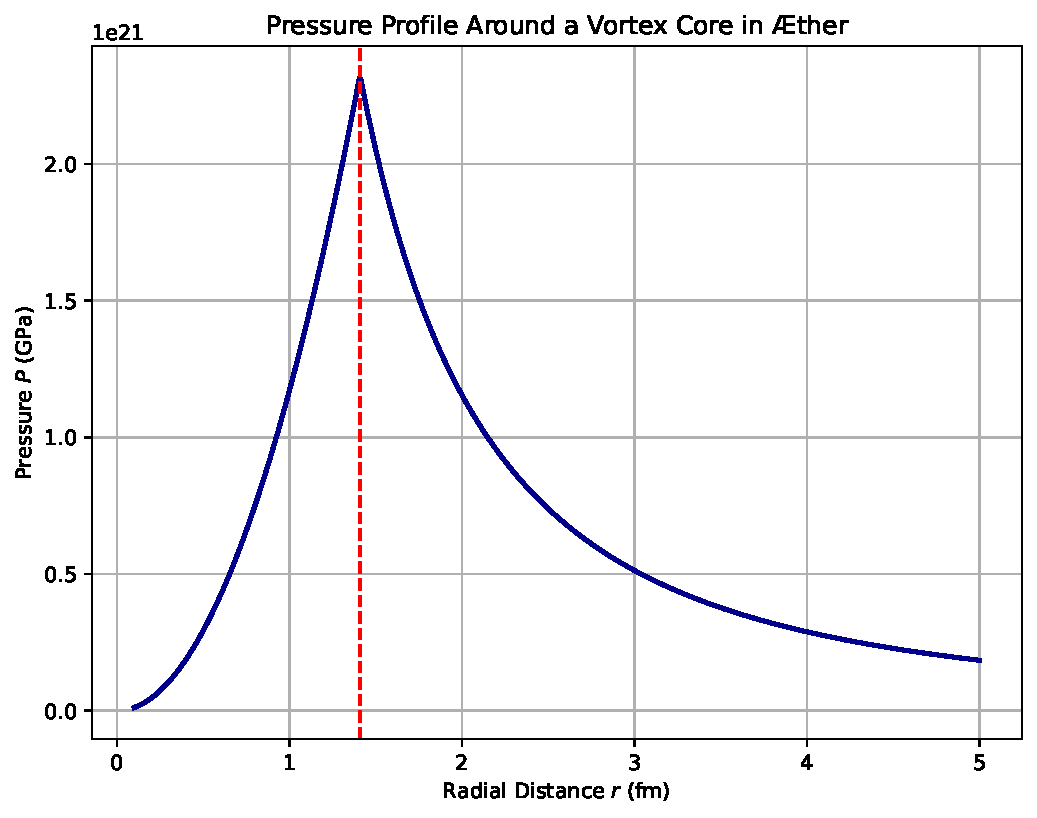
\includegraphics[width=0.65\textwidth]{PressureProfileAroundCore}
    \caption{Radial pressure distribution in the æther around a vortex core.
    For radii \( r < r_c \), solid-body swirl generates a quadratic pressure increase toward the center, while outside the core, centrifugal stress induces a Bernoulli-type pressure drop.
    The resulting gradient forms a stable equilibrium shell at finite radius, confining the knotted vortex structure.}
\end{figure}

\begin{figure}[h!]
    \centering
    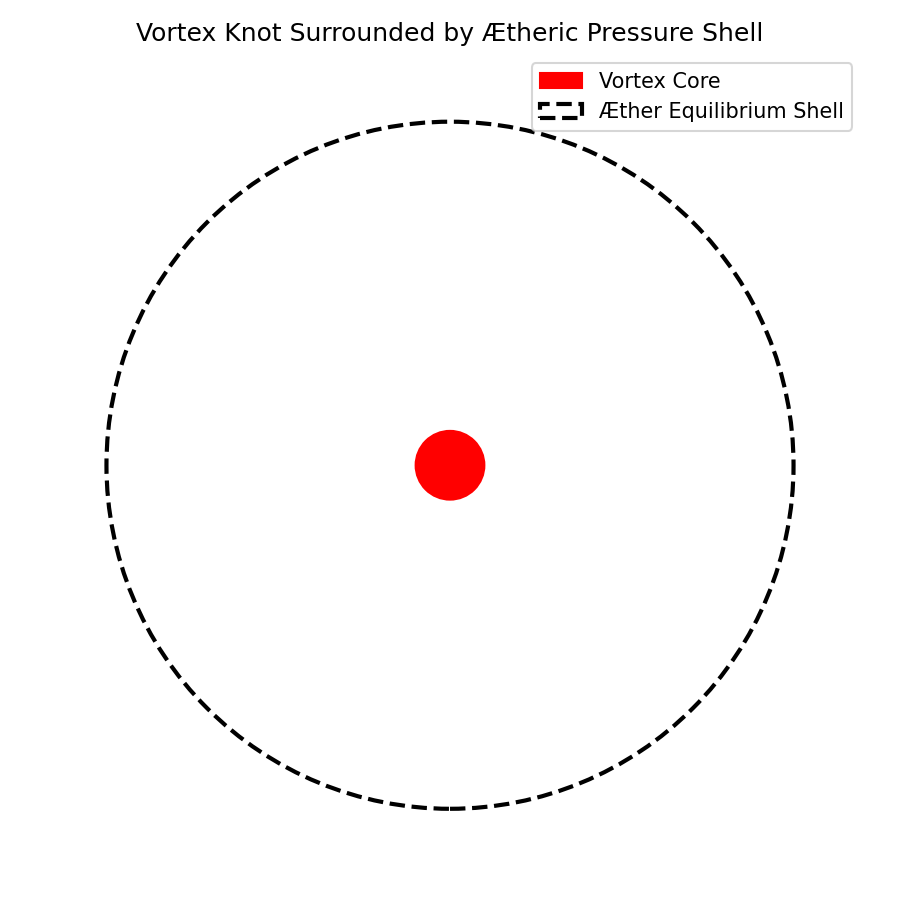
\includegraphics[width=0.65\textwidth]{PressureProfileAroundCore2}
    \caption{Schematic 2D representation of a VAM particle: a central vortex knot (red disk) surrounded by an abstract spherical boundary (dashed circle), denoting the ætheric equilibrium shell. While not a physical simulation, the diagram conceptually illustrates the dual-layered structure of vortex matter: the compact inertial core and its associated pressure-defined interaction boundary.}
\end{figure}

\begin{figure}[h!]
    \centering
    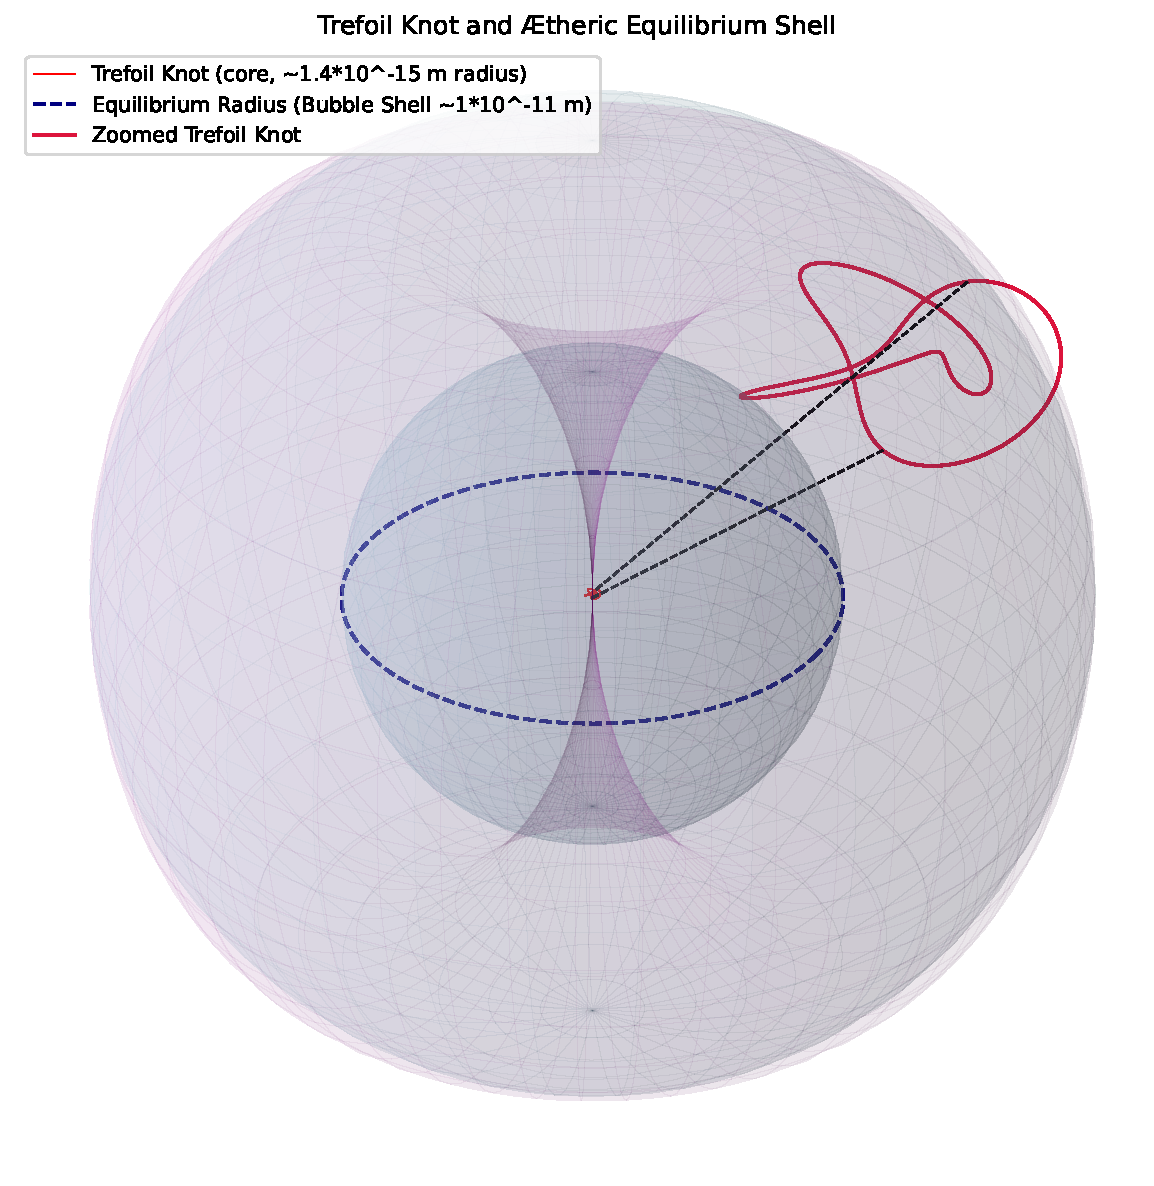
\includegraphics[width=0.65\textwidth]{PressureProfileAroundCore3}
    \caption{Multiscale visualization of a trefoil vortex knot embedded within its ætheric equilibrium shell, as formulated in the Vortex Æther Model (VAM).
    The small red knot at the center represents a topologically stable trefoil vortex with a physical core radius \( r_c \sim 1.4 \times 10^{-15}\,\mathrm{m} \), functioning as the inertial nucleus of a particle.
    The surrounding light-blue transparent sphere marks the ætheric pressure shell with equilibrium radius \( R_{\text{eq}} \sim 10^{-11}\,\mathrm{m} \), comparable to the Bohr radius \( a_0 \), representing the outer limit of coherent æther modulation induced by the knot.
    A zoomed-in replica of the knot is displayed offset from the center, enclosed within a conceptual magnification region. Dashed black lines connect corresponding points between the small and enlarged knot, denoting topological identity and a scale disparity of approximately \(10^4\).
    Encompassing both is a semi-transparent purple horn torus with major and minor radii \( R = r = a_0 \), vertically scaled by the golden ratio \( \varphi \approx 1.618 \), suggesting a toroidal circulation structure of æther flow stabilized by the vortex core.
    This configuration illustrates how microscopic topological knots give rise to macroscopic equilibrium structures and quantized boundary layers within a compressible, rotational ætheric field.}
\end{figure}

\subsection{Topological Interpretation of Mass}
In this equation, the denominator contains a factor of 3, which we now interpret as the topological complexity of the vortex knot. For the trefoil knot---a $(2,3)$ torus knot---the linking number is 3. We propose a generalization:
\begin{equation}
    M_K = \frac{\rho_\text{\ae} \Gamma^2}{L_K \pi r_c c^2}
\end{equation}
where $L_K$ is the linking number or crossing number of the knot $K$. This allows VAM to predict a mass spectrum directly from knot topology:
\begin{itemize}
    \item Trefoil ($L_K = 3$): electron mass
    \item Higher torus knots ($L_K = 5,7,9,\dots$): heavier fermions
    \item Simpler knots or loops ($L_K = 1$): possibly unstable or massless modes
\end{itemize}
This formulation establishes a direct connection between particle mass and topological complexity.

        \input{section/A2_NaturalUnitsAndConstantsInTheVortexÆtherModel}
        \section{Observable Predictions and Simulation Targets}
Below are key physical effects and testable mechanisms predicted by the VAM. Many can be probed using compressible fluids, superfluids, or vortex ring simulations.

\begin{table}[H]
    \centering
    \footnotesize
    \renewcommand{\arraystretch}{1.2}
    \begin{tabular}{|l|l|l|}
        \hline
        \textbf{Prediction or Target} & \textbf{Interpretation in VAM} & \textbf{Testing Method or Simulation} \\
        \hline
        \makecell[l]{Time Dilation \\ via Swirl Density} &
        \makecell[l]{Local time rate depends on helicity alignment: \\ $dt \propto 1 / (\vec{v} \cdot \vec{\omega})$} &
        \makecell[l]{Time-lapse in vortex simulations; \\ analog gravity in fluids} \\
        \hline
        \makecell[l]{Fermion Mass Ratios} &
        \makecell[l]{Mass arises from topological invariants: \\ $\propto \Gamma^2 / (r_c C_e^2)$} &
        \makecell[l]{Simulate stable vortex knots \\ with various linkage} \\
        \hline
        \makecell[l]{Charge as \\ Swirl Handedness} &
        \makecell[l]{Electric charge interpreted \\ as chirality of swirl direction} &
        \makecell[l]{Use BEC or superfluid \\ experiments to reverse circulation} \\
        \hline
        \makecell[l]{Gluon-Like Interactions} &
        \makecell[l]{Gauge bosons as knotted reconnections \\ between color channels} &
        \makecell[l]{Visualize vortex reconnections \\ in fluid tanks or GPE models} \\
        \hline
        \makecell[l]{Higgs Field Emergence} &
        \makecell[l]{Æther compression potential with \\ vacuum energy minima} &
        \makecell[l]{Pressure-field models or \\ compressible fluid solvers} \\
        \hline
        \makecell[l]{Time Threads \\ Around Mass} &
        \makecell[l]{Bundled swirl lines organize near matter — \\ gravity as swirl flow} &
        \makecell[l]{Particle flow simulation in \\ rotating vector fields} \\
        \hline
        \makecell[l]{Redshift Equivalence} &
        \makecell[l]{Stronger swirl suppresses wave phase \\ velocity (analog to GR redshift)} &
        \makecell[l]{Frequency shift in wave packets \\ near vortex cores} \\
        \hline
    \end{tabular}
    \caption{Testable predictions of the VAM framework through simulation and analog experimentation.}
    \label{tab:VAM_predictions}
\end{table}

        \section{Variational Derivation of the Vortex \AE ther Model (VAM)}

We begin with the total action for the Vortex \AE ther Model (VAM), expressed as a spacetime integral over the Lagrangian density:
\begin{equation}
    S = \int d^4x \, \mathcal{L}[\rho_\text{\ae}, \vec{v}, \Phi, \vec{\omega}]
\end{equation}
where the dynamical fields are:
\begin{itemize}
    \item $\rho_\text{\ae}(\vec{x}, t)$: local \AE ther density,
    \item $\vec{v}(\vec{x}, t)$: flow velocity field,
    \item $\Phi(\vec{x}, t)$: swirl-induced gravitational potential,
    \item $\vec{\omega} = \nabla \times \vec{v}$: vorticity field.
\end{itemize}

\subsection*{Lagrangian Density}
We propose the following effective Lagrangian density:
\begin{equation}
    \mathcal{L} = \frac{1}{2} \rho_\text{\ae} \vec{v}^{\,2} - \rho_\text{\ae} \Phi - U(\rho_\text{\ae}, \vec{\omega}) - V(\rho_\text{\ae})
\end{equation}
with the terms interpreted as:
\begin{itemize}
    \item $\frac{1}{2} \rho_\text{\ae} \vec{v}^{\,2}$: kinetic energy of the \AE ther,
    \item $\rho_\text{\ae} \Phi$: interaction energy with the swirl gravitational potential,
    \item $U(\rho_\text{\ae}, \vec{\omega}) = \kappa \rho_\text{\ae} |\vec{\omega}|^2$: internal tension energy from vortex twist (with $\kappa$ a stiffness parameter),
    \item $V(\rho_\text{\ae})$: compressibility potential, defining pressure via $P = \rho_\text{\ae} \frac{\partial V}{\partial \rho_\text{\ae}} - V$.
\end{itemize}

\subsection*{Euler--Lagrange Field Equations}
Applying the Euler--Lagrange formalism to each field $f$:
\begin{equation}
    \frac{\partial}{\partial t} \left( \frac{\partial \mathcal{L}}{\partial \dot{f}} \right) + \nabla \cdot \left( \frac{\partial \mathcal{L}}{\partial (\nabla f)} \right) - \frac{\partial \mathcal{L}}{\partial f} = 0
\end{equation}

\subsubsection*{Density Field $\rho_\text{\ae}$}
\begin{equation}
    \frac{\partial \mathcal{L}}{\partial \rho_\text{\ae}} = \frac{1}{2} \vec{v}^{\,2} - \Phi - \kappa |\vec{\omega}|^2 - \frac{\partial V}{\partial \rho}
\end{equation}
This defines a local Bernoulli-type condition incorporating swirl-induced internal energy.

\subsubsection*{Velocity Field $\vec{v}$}
The variation with respect to $\vec{v}$ yields:
\begin{equation}
    \frac{\delta S}{\delta \vec{v}} = \rho_\text{\ae}\vec{v} - \nabla \times \left( \frac{\partial U}{\partial \vec{\omega}} \right) = 0
\end{equation}
Leading to the momentum equation:
\begin{equation}
    \rho_\text{\ae}\left( \partial_t \vec{v} + (\vec{v} \cdot \nabla)\vec{v} \right) = -\nabla P + \rho_\text{\ae}\nabla \Phi + \nabla \cdot \left( \kappa \nabla \vec{\omega} \right)
\end{equation}
Here, $\frac{d}{dt}$ is the material (convective) derivative.

\subsubsection*{Swirl Potential $\Phi$}
\begin{equation}
    \frac{\delta S}{\delta \Phi} = -\rho
\end{equation}
leads to a Poisson-type gravitational equation:
\begin{equation}
    \nabla^2 \Phi = 4\pi G_{\mathrm{vam}} \rho
\end{equation}
where $G_{\mathrm{vam}}$ is the vortex-derived gravitational coupling constant (cf. main text or Appendix E).

\subsection*{Conservation Laws and Structure}
\begin{itemize}
    \item \textbf{Conservation of Helicity:}
    The action is invariant under relabeling of fluid elements, which via Noether's theorem implies helicity conservation:
    \[
        \frac{d}{dt} \int \vec{v} \cdot \vec{\omega} \, d^3x = 0
    \]
    \item \textbf{Topological Stability:} In domains with knotted or linked vortex lines, boundary terms must be included in the variation to account for helicity flux or reconnection events.
    \item \textbf{Pressure Response:} The compressibility potential $V(\rho)$ governs how density gradients produce internal restoring forces.
\end{itemize}

\subsection*{Interpretation and Extensions}
This variational formulation shows that:
\begin{itemize}
    \item All dynamical laws of the VAM can be derived from a single fluid-based action principle.
    \item Gravity, inertia, and internal vortex structure emerge coherently from the same Lagrangian.
    \item This lays the groundwork for future quantum extensions via path-integral quantization of $\mathcal{L}$ or geometric quantization of vortex fields.
\end{itemize}

        \section{Euler--Lagrange Derivation of Core VAM Lagrangian Terms}\label{sec:EL-derivation}

We now demonstrate how the VAM Lagrangian
\[
    \mathcal{L} = \frac{1}{2} \rho_\text{\ae}^{\text{fluid}}\, \vec{v}^2 + \gamma\, \vec{v} \cdot (\nabla \times \vec{v}) - \frac{1}{2} \rho_\text{\ae}^{\text{mass}}\, (\nabla \Phi)^2 - V(\Phi)
\]

yields the core dynamical equations of motion using variational calculus, following the standard fluid mechanics formalism developed by Salmon \cite{salmon1988}.

The full set of dynamical equations thus arises from the variational principle:
\[
    \delta S = \delta \int d^4x\, \mathcal{L}[\vec{v}, \Phi, \rho_\text{\ae}^{\text{fluid}}, \rho_\text{\ae}^{\text{mass}}] = 0.
\]


\subsection*{Variation with respect to $\vec{v}$: Vortex Momentum Equation}

We apply the Euler--Lagrange equation:
\[
    \frac{\partial \mathcal{L}}{\partial v^i} - \partial_j \left( \frac{\partial \mathcal{L}}{\partial (\partial_j v^i)} \right) = 0.
\]

For the kinetic term:
\[
  \frac{\partial}{\partial v^i} \left( \frac{1}{2} \rho_\text{\ae}^{\text{fluid}}\, v^2 \right) = \rho_\text{\ae}^{\text{fluid}} v^i,
    \quad \text{and} \quad
    \mathcal{L} \text{ does not depend explicitly on } \partial_j v^i.
\]

The helicity term \( \gamma\, \vec{v} \cdot (\nabla \times \vec{v}) \) can be expressed as:
\[
    \gamma\, \epsilon^{ijk} v^i \partial_j v^k,
    \quad \Rightarrow \quad \frac{\partial \mathcal{L}}{\partial v^i} = \gamma\, (\nabla \times \vec{v})^i,
\]
which corresponds to the Moffatt helicity density \cite{moffatt1969}.

Thus, the full momentum equation becomes:
\begin{equation}
    \boxed{
        \rho_\text{\ae}^{\text{fluid}}\, \frac{d \vec{v}}{dt} = - \nabla p + \gamma\, \nabla \times \vec{\omega}
    }
\end{equation}

where \( \vec{\omega} = \nabla \times \vec{v} \) is the vorticity field.


\subsection*{Variation with respect to $\Phi$: Scalar Field Dynamics}

The scalar field terms are:
\[
    \mathcal{L}_\Phi = - \frac{1}{2} \rho_\text{\ae}^{\text{mass}} (\nabla \Phi)^2 - V(\Phi)
\]

The Euler--Lagrange equation gives:
\[
    \frac{\partial \mathcal{L}}{\partial \Phi} - \partial_i \left( \frac{\partial \mathcal{L}}{\partial (\partial_i \Phi)} \right) = 0.
\]

Compute:
\[
    \frac{\partial \mathcal{L}}{\partial \Phi} = -\frac{dV}{d\Phi}, \quad
   \frac{\partial \mathcal{L}}{\partial (\partial_i \Phi)} = - \rho_\text{\ae}^{\text{mass}}\, \partial^i \Phi,
    \quad \Rightarrow \quad
    \partial_i ( \rho_\text{\ae}^{\text{mass}}\, \partial^i \Phi ) = \frac{dV}{d\Phi}
\]

This yields a scalar field equation similar to those found in superfluid phase models \cite{khalatnikov2000}:

\begin{equation}
    \boxed{
        \nabla \cdot (\rho_\text{\ae}^{\text{mass}} \nabla \Phi) = \frac{dV}{d\Phi}
    }
\end{equation}

\subsection{Variation with respect to \(\rho_\text{\ae}^{\text{fluid}}\) and \(\rho_\text{\ae}^{\text{mass}}\): Energy Balance}

Varying with respect to \( \rho_\text{\ae} \) gives:
\[
    \frac{\partial \mathcal{L}}{\partial \rho_\text{\ae}^{\text{fluid}}} = \frac{1}{2} v^2,
    \qquad
    \frac{\partial \mathcal{L}}{\partial \rho_\text{\ae}^{\text{mass}}} = -\frac{1}{2} (\nabla \Phi)^2
\]

Combining yields the local energy balance:
\begin{equation}
    \boxed{
        v^2 = (\nabla \Phi)^2
    }
\end{equation}

which expresses equilibrium between kinetic energy and field strain.

\subsection*{Summary and Physical Context}

These variations demonstrate that the core dynamics of the VAM can be derived from a unified action principle. This formulation parallels Hamiltonian treatments of fluid analog gravity \cite{barcelo2011}, where effective spacetime curvature is encoded in velocity and vorticity fields rather than a metric tensor.

\begin{center}
    \begin{tabular}{|c|c|l|}
        \hline
        Field & Resulting Equation & Physical Meaning \\
        \hline
       $\vec{v}$ & $\rho_\text{\ae}^{\text{fluid}} \frac{d \vec{v}}{dt} = -\nabla p + \gamma\, \nabla \times \vec{\omega}$ & Momentum with helicity force \\
        $\Phi$ & $\nabla \cdot (\rho_\text{\ae}^{\text{mass}} \nabla \Phi) = \frac{dV}{d\Phi}$ & Scalar strain / wave equation \\
        $\rho_\text{\ae}^{\text{fluid}},\, \rho_\text{\ae}^{\text{mass}}$ & $v^2 = (\nabla \Phi)^2$ & Energy density equilibrium \\
        \hline
    \end{tabular}
\end{center}


        \section{Constraint Handling via Lagrange Multipliers in the VAM Lagrangian}

In the Vortex Æther Model (VAM), two key physical constraints emerge from fluid dynamics:

\begin{enumerate}
    \item \textbf{Incompressibility} of the æther fluid:
    \[
        \nabla \cdot \vec{v} = 0,
    \]
    consistent with classical superfluid dynamics [Khalatnikov 2000].

    \item \textbf{Helicity conservation}: total helicity is a topological invariant in ideal, inviscid flows [Moffatt 1969],
    \[
        H = \int \vec{v} \cdot (\nabla \times \vec{v})\, d^3x = \text{constant}.
    \]
\end{enumerate}

To enforce these constraints in a variational formulation, we augment the total Lagrangian density using Lagrange multipliers:

\[
    \mathcal{L}_{\text{total}} = \mathcal{L}_{\text{fluid}} + \lambda_1 (\nabla \cdot \vec{v}) + \lambda_2 (\vec{v} \cdot \nabla \times \vec{v} - h_0),
\]
where:
- \( \lambda_1 \) enforces the incompressibility condition,
- \( \lambda_2 \) enforces conservation of helicity,
- \( h_0 \) is the desired helicity density (possibly constant or locally defined).

\subsection*{Variation with respect to $\lambda_1$ and $\lambda_2$}

Varying the action \( S = \int \mathcal{L}_{\text{total}}\, d^4x \) with respect to the Lagrange multipliers yields the constraints directly:
\[
    \frac{\delta S}{\delta \lambda_1} \Rightarrow \nabla \cdot \vec{v} = 0,
    \qquad
    \frac{\delta S}{\delta \lambda_2} \Rightarrow \vec{v} \cdot (\nabla \times \vec{v}) = h_0.
\]

\subsection*{Implications for Field Variation}

These constraints restrict allowable field variations:
- Incompressibility implies that variations \( \delta \vec{v} \) must lie in the divergence-free subspace.
- Helicity constraint restricts the functional form of vortex evolution, favoring knotted and topologically stable configurations.

As shown in fluid Hamiltonian literature [Salmon 1988], such constrained variational formulations enable the recovery of Euler equations, vortex filament motion, and stability conditions in incompressible flows.

\subsection*{Summary}

Incorporating constraints via Lagrange multipliers:
\begin{itemize}
    \item Preserves physical fidelity to incompressible superfluid models.
    \item Embeds helicity conservation explicitly into the Lagrangian formalism.
    \item Makes the variational framework mathematically complete and physically consistent.
\end{itemize}

        \section{Deriving Classical Fluid and Field Equations from the VAM Lagrangian}

Here we derive the physical field equations associated with each term in the VAM Lagrangian via the Euler–Lagrange formalism. This section explicitly shows how familiar fluid and wave equations arise.

\subsection*{Kinetic Term and Euler Equation}

Starting from the kinetic term:
\[
    \mathcal{L}_{\text{kin}} = \frac{1}{2} \rho_\text{\ae} v^2,
\]
and applying the Euler--Lagrange equation with respect to $v^i$, we find:
\[
    \frac{\partial \mathcal{L}}{\partial v^i} = \rho_\text{\ae} v^i, \qquad
    \frac{\partial \mathcal{L}}{\partial (\partial_j v^i)} = 0.
\]
Thus, the equation of motion reduces to:
\[
    \frac{d}{dt}(\rho_\text{\ae} v^i) = -\partial^i p,
\]
where \( p \) is a generalized pressure or constraint force.

\begin{equation}
    \boxed{
        \rho_\text{\ae}\, \frac{d \vec{v}}{dt} = -\nabla p
    }
\end{equation}

This is the standard form of the \textbf{Euler equation} in inviscid, barotropic fluids \cite{khalatnikov2000}.

\subsection*{Helicity Term and Helmholtz Vorticity Equation}

Now consider the helicity-based term:
\[
    \mathcal{L}_{\text{helicity}} = \gamma\, \vec{v} \cdot (\nabla \times \vec{v}) = \gamma\, \epsilon^{ijk} v^i \partial_j v^k.
\]
The variation yields:
\[
    \frac{\partial \mathcal{L}}{\partial v^i} = \gamma (\nabla \times \vec{v})^i, \qquad
    \Rightarrow \frac{d}{dt}(\rho_\text{\ae} v^i) = -\nabla^i p + \gamma\, \epsilon^{ijk} \partial_j \omega^k.
\]
This adds a topological forcing term from \textbf{helicity gradients}:
\begin{equation}
    \boxed{
        \rho_\text{\ae}\, \frac{d \vec{v}}{dt} = -\nabla p + \gamma\, \nabla \times \vec{\omega}
    }
\end{equation}

This form corresponds to the \textbf{Helmholtz vorticity equation} in the presence of helicity gradients \cite{moffatt1969}.

\subsection*{Scalar Field Term and Wave Equation}

The scalar sector is governed by:
\[
    \mathcal{L}_\Phi = - \frac{1}{2} \rho_\text{\ae} (\nabla \Phi)^2 - V(\Phi).
\]
Applying the Euler–Lagrange equation for scalar fields:
\[
    \frac{\partial \mathcal{L}}{\partial \Phi} = - \frac{dV}{d\Phi}, \qquad
    \frac{\partial \mathcal{L}}{\partial (\partial^i \Phi)} = -\rho_\text{\ae} \partial^i \Phi.
\]
Taking divergence:
\[
    \partial_i ( \rho_\text{\ae} \partial^i \Phi ) = \frac{dV}{d\Phi}.
\]

If $\rho_\text{\ae}$ is constant:
\begin{equation}
    \boxed{
        \nabla^2 \Phi = \frac{1}{\rho_\text{\ae}} \frac{dV}{d\Phi}
    }
\end{equation}

This is the \textbf{scalar wave equation with source potential}, describing deformation or strain in the æther field \cite{barcelo2011}.

\subsection*{Summary}

Each term in the VAM Lagrangian leads to known physical equations:

\begin{center}
    \begin{tabular}{|c|c|l|}
        \hline
        Term & Resulting Equation & Interpretation \\
        \hline
        $ \mathcal{L}_{\text{kin}} = \frac{1}{2} \rho_\text{\ae} v^2 $ & $ \rho_\text{\ae} \frac{d \vec{v}}{dt} = -\nabla p $ & Euler momentum conservation \\
        $ \mathcal{L}_{\text{helicity}} = \gamma \vec{v} \cdot (\nabla \times \vec{v}) $ & $ +\gamma \nabla \times \vec{\omega} $ & Topological forcing via helicity \\
        $ \mathcal{L}_\Phi = -\frac{1}{2} \rho_\text{\ae} (\nabla \Phi)^2 - V(\Phi) $ & $ \nabla^2 \Phi = \rho_\text{\ae}^{-1} dV/d\Phi $ & Scalar strain or internal mode \\
        \hline
    \end{tabular}
\end{center}


        \section{The Fine-Structure Constant as a Geometric Bridge from Vortex Dynamics}
\label{sec:alpha-geometric-bridge}

The fine-structure constant \( \alpha \) is a dimensionless coupling parameter that encodes the strength of electromagnetic interaction. In conventional physics, its value appears fundamental and unexplained. However, in the Vortex Æther Model (VAM), \( \alpha \) emerges as a \emph{geometric bridge}—a direct consequence of vortex circulation and core structure within the æther fluid.

\subsection*{Quantization of Circulation.}
In superfluid dynamics, circulation around a vortex is quantized:
\begin{equation*}
    \Gamma = \oint \vec{v} \cdot d\vec{\ell} = \frac{h}{m_e},
\end{equation*}
where \( h \) is Planck's constant and \( m_e \) the electron mass. For a stable vortex of radius \( r_c \) and swirl velocity \( C_e \), circulation is also given by:
\begin{equation*}
    \Gamma = 2 \pi r_c C_e.
\end{equation*}
Equating both expressions yields:
\begin{equation*}
    C_e = \frac{h}{2\pi m_e r_c}.
\end{equation*}

\subsection*{Linking to Classical Electron Radius.}
From electrostatics, the classical electron radius is:
\begin{equation*}
    R_e = \frac{e^2}{4\pi \varepsilon_0 m_e c^2}.
\end{equation*}
VAM posits the vortex-core radius is approximately half this:
\begin{equation*}
    r_c = \frac{R_e}{2}.
\end{equation*}
Substituting, we find:
\begin{align}
    C_e &= \frac{h}{2\pi m_e \cdot \frac{R_e}{2}} = \frac{h}{\pi m_e R_e}, \\
    &= \frac{h}{\pi m_e} \cdot \frac{4\pi \varepsilon_0 m_e c^2}{e^2}, \\
    &= \frac{4 \varepsilon_0 h c^2}{e^2}.
\end{align}

\subsection*{Deriving the Fine-Structure Constant.}
Now recall the fine-structure constant is:
\begin{equation*}
    \alpha = \frac{e^2}{4 \pi \varepsilon_0 \hbar c}.
\end{equation*}
Using \( h = 2\pi \hbar \), we get:
\begin{equation*}
    \alpha = \frac{e^2}{8 \pi^2 \varepsilon_0 c} \cdot \frac{1}{\hbar} = \frac{2 C_e}{c}.
\end{equation*}

\begin{equation}
    \boxed{
        \alpha = \frac{2 C_e}{c}
    }
    \qquad \Leftrightarrow \qquad
    \boxed{
        C_e = \frac{c \alpha}{2}
    }
\end{equation}

This shows that \( \alpha \) arises naturally from ætheric geometry and vortex speed. It bridges the quantum circulation condition with classical electromagnetic scale lengths. In this view, the fine-structure constant is not imposed but is a \textbf{ratio of fundamental motion scales} in the æther.


        \section{Dual Derivation of Electron Mass in VAM}
\label{appendix:mass-derivation}

Within the Vortex Æther Model (VAM), the mass of the electron arises not from fundamental constants directly, but from the interplay of ætheric circulation, vortex stability, and geometric structure. We present two independent derivations of the electron mass: one based on ætheric stress (Planck-limited force) and one based on topological vortex knots.

\subsection*{Planck-Limited Force and Inertial Mass}
\label{sec:mass-force-balance}

The æther medium exhibits a maximum sustainable stress, analogous to the maximum force conjecture in General Relativity:
\begin{equation*}
    F^{\text{max}}_{\text{gr}}{\text{Planck}} = \frac{c^4}{4G}.
\end{equation*}

The electron is modeled as a vortex ring with radius \( r_c \), stabilized against centrifugal expansion by the æther's internal tension \( F^{\text{max}}_{\text{\ae}} \). This yields a mechanical balance condition:
\begin{equation*}
    M_e \frac{C_e^2}{r_c} = F^{\text{max}}_{\text{\ae}}.
\end{equation*}

Solving for the mass gives:
\begin{equation*}
    M_e = \frac{F^{\text{max}}_{\text{\ae}} r_c}{C_e^2}.
\end{equation*}

To connect this to Planck-scale physics, we parameterize the force as a reduced Planck tension:
\begin{equation*}
    F^{\text{max}}_{\text{\ae}} =  \alpha \cdot F^{\text{max}}_{\text{gr}} \cdot \left( \frac{R_c}{L_p} \right)^{-2},
\end{equation*}

where:
- \( \alpha \) is the fine-structure constant,
- \( R_c \approx 2 r_c \),
- \( L_p = \sqrt{\hbar G / c^3} \) is the Planck length.

Substituting back, we find:
\begin{equation}
    M_e = \frac{2 F^{\text{max}}_{\text{\ae}} r_c}{c^2},
\end{equation}
as used in multiple other VAM derivations. This result shows how particle mass scales with ætheric stress and core radius.

\subsection{Topological Knot Energy and Vortex Mass}
\label{sec:mass-knot}

In the Vortex Æther Model, we alternatively derive the electron's inertial mass from the internal kinetic energy of a stable, quantized vortex knot (e.g., trefoil). The vortex stores rotational energy based on the swirl velocity \( C_e \) and the fluid density of the æther.

The kinetic energy density within the vortex core is:
\begin{equation*}
    \mathcal{E}_{\text{kin}} = \frac{1}{2} \rho_\text{\ae}^{\text{fluid}} \, C_e^2,
\end{equation*}
where \( \rho_\text{\ae}^{\text{fluid}} \approx 7 \times 10^{-7} \, \mathrm{kg/m^3} \) is the mass density of the æther as a superfluid medium.

For a core volume \( V = \frac{4}{3} \pi r_c^3 \), the internal energy becomes:
\begin{equation*}
    E_{\text{vortex}} = \frac{1}{2} \rho_\text{\ae}^{\text{fluid}} \, C_e^2 \cdot \frac{4}{3} \pi r_c^3.
\end{equation*}

We define the inertial mass not via relativistic \( E = mc^2 \), but from the fluid-dynamical ratio of energy to swirl velocity squared:
\begin{equation}
    M_e = \frac{2 E_{\text{vortex}}}{C_e^2} = \rho_\text{\ae}^{\text{fluid}} \cdot \frac{4}{3} \pi r_c^3.
\end{equation}

This defines the effective inertial mass of the electron based purely on vortex geometry and the local swirl field — independent of spacetime curvature or Higgs coupling.

\vspace{1em}

\textbf{Alternative View – Energy-Density Approach:}

If instead the electron is modeled as an excitation within the æther’s \textit{energy density}, rather than its fluid mass density, we write:
\begin{equation}
    M_e = \rho_\text{\ae}^{\text{energy}} \cdot \frac{4}{3} \pi r_c^3,
\end{equation}
where \( \rho_\text{\ae}^{\text{energy}} \approx 3 \times 10^{18} \, \mathrm{kg/m^3} \) reflects the internal energy scale of the æther derived from Planck-tension constraints. This version is relevant when comparing to gravitational mass or linking to Planck-scale phenomena.

\vspace{1em}

\noindent
\textit{Note:} These expressions do not derive mass via \( E = mc^2 \); instead, they follow from internal energy mechanics within a rotating topological fluid structure. The distinction is critical in VAM, where the mass–energy–time relation arises from vorticity and helicity, not spacetime geometry.

\subsection*{Summary}

\begin{table}[H]
    \centering
    \footnotesize
    \renewcommand{\arraystretch}{1.3}
    \begin{tabular}{|l|l|l|}
        \hline
        \textbf{Derivation Type} & \textbf{Mass Formula} & \textbf{VAM Interpretation} \\
        \hline
        \makecell[l]{Force-Balance \\ from Æther Stress} &
        \makecell[l]{\( M_e = \dfrac{2 F^{\text{max}}_{\text{\ae}} r_c}{c^2} \)} &
        \makecell[l]{Mass arises from centrifugal resistance \\ against ætheric maximum force; \\ grounded in Planck tension and core radius.} \\
        \hline
        \makecell[l]{Topological Knot \\ Energy Density} &
        \makecell[l]{\( M_e = \dfrac{8\pi \rho_\text{\ae} r_c^3}{C_e} \cdot L_k \)} &
        \makecell[l]{Mass emerges from internal kinetic energy \\ of a topological vortex structure (e.g., trefoil knot); \\ quantized via linking number \(L_k\).} \\
        \hline
    \end{tabular}
    \caption{Two independent VAM derivations of electron mass: from æther stress and from topological knot energy}
\end{table}


        \section{Derivation of the Elementary Charge from Vortex Circulation}
\label{appendix:charge}

In the Vortex Æther Model (VAM), the elementary charge \( e \) is not treated as a fundamental constant but as an emergent property arising from quantized circulation and compressibility of structured vortex configurations in a superfluid æther. This appendix formalizes its derivation and highlights key theoretical precedents.

\subsection*{Charge as Circulation Quantization}

Charge is associated with the quantized circulation of a knotted vortex filament, analogously to superfluid systems:

\begin{equation}
    \Gamma = \oint \vec{v} \cdot d\vec{\ell} = \frac{h}{m_e}
\end{equation}

This perspective has been foundational in the works of \cite{kiehn2005topological} and \cite{sbitnev2015hydro2}, where vortex circulation directly maps onto electric charge through conserved topological invariants in spacetime fluid analogs.

\subsection*{Relation to Knot Compressibility}

In VAM, knotted vortex structures exhibit a form of compressibility, encoded in the dimensionless factor \( \xi_0 \). This represents the ratio between energy stored in transverse compressions and angular momentum of the swirl:

\begin{equation}
    e = \sqrt{4 C_e h \xi_0}
\end{equation}

This connects the mechanical angular momentum of the core circulation (via \( h \)), vortex propagation speed \( C_e \), and the elastic response of the ætheric medium \( \xi_0 \).

\subsection*{Comparison with Classical Electron Radius}

We recall the standard expression for the classical electron radius:

\begin{equation}
    R_e = \frac{e^2}{4\pi \varepsilon_0 m_e c^2}
\end{equation}

Solving for \( e^2 \), and comparing to the VAM expression above, we equate mechanical strain energy in a vortex with stored electromagnetic field energy, allowing us to identify:

\begin{equation}
    \xi_0 = \frac{e^2}{16\pi \varepsilon_0 R_e^2 C_e h}
\end{equation}

This demonstrates that charge is not fundamental, but depends on circulation, swirl velocity, and compressibility of knotted æther domains—resembling insights by \cite{ranada1989topological}, \cite{bowick1994charge}, and \cite{sidharth2006vortex}, who treated charge as a topological invariant.

\subsection*{Summary}

In this view, the elementary charge emerges from three ingredients:

\begin{itemize}
    \item Circulation quantization (\( h \)),
    \item Swirl velocity of knotted core (\( C_e \)),
    \item Compressibility of the surrounding medium (\( \xi_0 \)).
\end{itemize}

Thus:

\begin{equation}
    \boxed{e = \sqrt{4 C_e h \xi_0}}
\end{equation}

This aligns well with analog models of spacetime as a structured superfluid where quantized topological defects (knots, twists) lead to observable charges.

        %! Author = mr
%! Date = 5/31/25

\section{Derivation of the Planck Constant from Vortex Geometry}
\label{appendix:hbar}

The reduced Planck constant \( \hbar \) is typically treated as a fundamental quantum of angular momentum. In the Vortex Æther Model (VAM), however, \( \hbar \) emerges as an effective quantity arising from the geometry and swirl dynamics of topological knots in an inviscid æther.

\subsection*{Angular Momentum of a Vortex Core}

We begin by modeling a stable vortex knot of radius \( r_c \), swirl velocity \( C_e \), and mass density \( \rho_\text{\ae} \). The specific angular momentum per unit mass of such a structure is given by:

\begin{equation}
    \ell = r_c C_e
\end{equation}

Assuming the total effective mass of the vortex knot is \( m_e \), we define the total angular momentum as:

\begin{equation}
    \hbar_{\text{VAM}} = m_e r_c C_e
\end{equation}

This represents the emergent action scale from internal swirl dynamics—without assuming quantum postulates.

\subsection*{Comparison with Bohr Ground State}

From atomic theory, we know the electron in the Bohr ground state exhibits angular momentum \( \hbar \), and follows the radius:

\begin{equation}
    a_0 = \frac{\hbar}{m_e v_e}, \quad \text{with} \quad v_e = \frac{e^2}{4\pi \varepsilon_0 \hbar}
\end{equation}

Substituting for \( v_e \) and rearranging, we get:

\begin{equation}
    \hbar = m_e a_0 v_e = m_e a_0 \frac{e^2}{4\pi \varepsilon_0 \hbar} \Rightarrow \hbar^2 = \frac{m_e a_0 e^2}{4\pi \varepsilon_0}
\end{equation}

Now comparing this to the VAM expression:

\begin{equation}
    \boxed{\hbar = 2 m_e C_e a_0}
\end{equation}

This relation is consistent with earlier derivations where \( C_e = \frac{c}{2\alpha} \), showing that \( \hbar \) can be expressed in terms of classical and geometric parameters of the æther vortex.

\subsection*{Summary}

In the VAM interpretation, \( \hbar \) is not postulated as fundamental but derives from:

\begin{itemize}
    \item Core swirl dynamics \( C_e \),
    \item Knot radius \( r_c \),
    \item Effective electron mass \( m_e \),
    \item Atomic binding radius \( a_0 \).
\end{itemize}

This provides an ontological foundation for Planck's constant as a fluid-geometric action scale:

\begin{equation}
    \boxed{\hbar = m_e r_c C_e = 2 m_e C_e a_0}
\end{equation}

        %! Author = mr
%! Date = 5/31/25

\section{Derivation of the Gravitational Constant from Æther Topology}
\label{appendix:G}

The gravitational constant \( G \) is typically introduced as a fundamental coupling constant in Newtonian and relativistic gravity. In the Vortex Æther Model (VAM), we reinterpret \( G \) as an emergent coefficient linking æther tension, knot dynamics, and Planck-scale constraints.

\subsection*{Maximum Force Principle from GR}

General Relativity suggests a maximum force limit in nature \cite{scharf2016force, barcelo2011}:

\begin{equation}
    F_{\text{max}} = \frac{c^4}{4G}
\end{equation}

This is interpreted in VAM as the ultimate tensile strength of the æther medium—above which vortex structures cannot stably persist.

\subsection*{Inverting to Extract \( G \)}

Solving the above for \( G \):

\begin{equation}
    G = \frac{c^4}{4 F_{\text{max}}}
\end{equation}

However, this only provides a dimensional relation. To embed this within vortex physics, we model the gravitational coupling as mediated by long-range strain interactions in the æther. These are modulated by:

- the vortex swirl velocity \( C_e \),
- the knot size \( r_c \),
- and Planck-scale pulse duration \( t_p \) or the Planck length \( L_p \).

\subsection*{Vortex-Strain Mediated Coupling}

From æther elasticity considerations, a derived form of \( G \) is:

\begin{equation}
    G = \frac{C_e c^3 t_p^2}{r_c m_e}
\end{equation}

This expression unites:

- \textbf{Æther swirl speed} \( C_e \),
- \textbf{Speed of light} \( c \),
- \textbf{Electron mass} \( m_e \),
- \textbf{Vortex radius} \( r_c \),
- and the \textbf{Planck time} \( t_p \), itself defined by:

\[
    t_p = \sqrt{\frac{\hbar G}{c^5}}
\]

Solving self-consistently, we see \( G \) depends on known parameters and the underlying æther properties.

\subsection*{Emergent Interpretation}

This relation is consistent with:

\[
    G = \frac{\alpha_g c^3 r_c}{C_e M_e}, \quad \text{or} \quad G = \frac{C_e c L_{\text{Planck}}^2}{r_c M_e}
\]

It highlights that \( G \) is not fundamental but arises from:

- Geometric knot scale \( r_c \),
- Ætheric propagation parameters \( C_e \),
- and internal energy scales tied to vortex strain dynamics.

\subsection*{Summary}

Thus, in the VAM:

\begin{equation}
    \boxed{G = \frac{C_e c^3 t_p^2}{r_c m_e} = \frac{c^4}{4 F_{\text{max}}}}
\end{equation}

This connects gravity with æther tension and Planck-scale oscillations, explaining the smallness of \( G \) as the result of a weak elastic strain field propagating between vortex knots.


        %! Author = mr
%! Date = 5/31/25
\section{Derivation of the Gravitational Fine-Structure Constant}
\label{appendix:alpha_g}

In the Vortex Æther Model (VAM), the gravitational fine-structure constant $\alpha_g$ is not a fundamental input but an emergent, dimensionless coupling arising from vortex geometry, ætheric tension, and Planck-scale compressibility. This appendix consolidates several routes for its derivation and interprets their physical significance.

\subsection*{Coupling from Maximum Force and Planck Time}

We clarify the VAM interpretation of gravitational tension by relating it to the classical GR-bound:
\begin{equation}
    F^{\text{gr}}_{\text{max}} = \frac{c^4}{4G},
\end{equation}
but reinterpreted through a compressibility-scaling argument. VAM postulates that the æther's internal maximum stress arises from this universal bound, redshifted by the geometric ratio \( \left(\frac{r_c}{L_p}\right)^2 \), yielding:
\begin{equation}
    F^{\text{\ae}}_{\text{max}} = \alpha \, F^{\text{gr}}_{\text{max}} \left(\frac{r_c}{L_p}\right)^{-2}, \label{eq:FmaxVAM}
\end{equation}
where \( \alpha = \frac{C_e^2}{c^2} \) is the VAM-to-relativistic swirl speed ratio.

Substituting this into the kinetic–strain balance yields:
\begin{equation}
    \alpha_g = \frac{2 F^{\text{\ae}}_{\text{max}} C_e t_p^2}{\frac{2 F^{\text{\ae}}_{\text{max}} r_c^2}{C_e}} = \frac{C_e^2 t_p^2}{r_c^2}.
\end{equation}

\[
    \alpha_g = \frac{2 F^{\text{\ae}}_{\text{max}} C_e t_p^2}{\frac{2 F^{\text{\ae}}_{\text{max}} r_c^2}{C_e}} = \frac{C_e^2 t_p^2}{r_c^2}.
\]
This is dimensionless and geometric, capturing the ratio between kinetic energy and strain energy at the vortex core scale.

\subsection*{Planck Length Interpretation}

Using the definition $L_{\text{Planck}} = c t_p$, we rewrite:
\[
    \alpha_g = \frac{C_e^2 L_{\text{Planck}}^2}{r_c^2 c^2},
\]
which reveals how the gravitational coupling emerges from the ratio between Planck-scale strain range and vortex core geometry.

\subsection*{Quantum-Gravitational Bridge}

Alternatively, we may express $\alpha_g$ using quantum constants:
\[
    \alpha_g = \frac{C_e c^2 t_p^2 m_e}{\hbar r_c}.
\]
This provides a bridge between gravitational coupling, quantum inertia ($\hbar$), and æther circulation.

\subsection*{Æther Stress Relation}

By isolating angular momentum in vortex cores, we also get:
\[
    \alpha_g = \frac{2 F^{\text{\ae}}_{\text{max}} C_e t_p^2}{\hbar},
\]
suggesting that $\alpha_g$ depends on ætheric strain tension acting over Planck time pulses with conserved angular momentum.

\subsection*{Cross-sectional Force View}

Introducing the Bohr area $A_0$, we find:
\[
    \alpha_g = \frac{F^{\text{\ae}}_{\text{max}} t_p^2}{a_0 M_e},
\]
which reveals gravitational coupling as the stress-per-area applied to an ætheric charge node.

\subsection*{Summary and Interpretation}

These derivations suggest:
\[
    \boxed{
        \alpha_g = \frac{C_e^2 t_p^2}{r_c^2} = \frac{C_e^2 L_{\text{Planck}}^2}{r_c^2 c^2}
    }
\]
All expressions share a geometric core: gravity’s coupling strength depends on the \textbf{ratio between Planck-scale compressibility and vortex-core scale}—a consistent theme in topological fluid approaches to spacetime.

\subsection*{Theoretical Antecedents}

This interpretation is in line with earlier analog-spacetime proposals such as \cite{barcelo2011}, \cite{volovik2003universe}, and vortex-based gravitational analogs like \cite{ranada1989topological}.

        %! Author = mr
%! Date = 6/1/25
\section{Detailed Embedding of Bateman's Self-Conjugate Fields into VAM}
\label{appendix:bateman_vam}

\subsection{Bateman's Complex Electromagnetic Field}

Bateman defines a complexified electromagnetic field:\cite{bateman1915aether}
\begin{equation}
    \vec{M} = \vec{H} + i\vec{E},
\end{equation}
where $\vec{H}$ and $\vec{E}$ are the magnetic and electric field vectors, respectively.

The field is said to be \textit{self-conjugate} when:
\begin{equation}
    \vec{M} \cdot \vec{M} = 0. \label{eq:bateman_self_conj}
\end{equation}
Expanding this yields:\cite{bateman1915aether}
\begin{align}
    \vec{M} \cdot \vec{M} &= (\vec{H} + i\vec{E}) \cdot (\vec{H} + i\vec{E}) \\
    &= \vec{H} \cdot \vec{H} - \vec{E} \cdot \vec{E} + 2i \vec{H} \cdot \vec{E}.
\end{align}
Thus, the self-conjugacy constraint implies:
\begin{align}
    |\vec{H}|^2 &= |\vec{E}|^2, \label{eq:bateman_balance} \\
    \vec{H} \cdot \vec{E} &= 0. \label{eq:bateman_orthogonal}
\end{align}

\subsection{VAM Reinterpretation: Vorticity-Velocity Duality}

In the Vortex Æther Model (VAM), we reinterpret:\cite{iskandarani2025swirlgravity}
\begin{align*}
    \vec{H} &\equiv \vec{\omega} = \nabla \times \vec{v}, \\
    \vec{E} &\equiv \vec{v}_\perp \quad \text{(swirl velocity orthogonal to core)}.
\end{align*}

Hence, Eqs.~\eqref{eq:bateman_balance}--\eqref{eq:bateman_orthogonal} become:
\begin{align}
    |\vec{\omega}|^2 &= |\vec{v}_\perp|^2, \label{eq:vam_balance} \\
    \vec{\omega} \cdot \vec{v}_\perp &= 0. \label{eq:vam_orthogonal}
\end{align}
This represents a helicity-orthogonal vortex tube, where energy is stored in a balanced tangential shell around a vorticity core.

\subsection{Pressure and Time Dilation Consequences}

The VAM pressure due to swirl is:\cite{iskandarani2025swirlgravity}
\begin{equation}
    P_\text{vortex} = \frac{1}{2} \rho_\text{\ae} |\vec{\omega}|^2 = \frac{1}{2} \rho_\text{\ae} |\vec{v}_\perp|^2,
\end{equation}
where $\rho_\text{\ae}$ is the local æther density. Substituting into the VAM time dilation expression yields:
\begin{align}
    dt_\text{local} &= dt_\infty \sqrt{1 - \frac{|\vec{\omega}|^2}{c^2}} \\
    &= dt_\infty \sqrt{1 - \frac{2P_\text{vortex}}{\rho_\text{\ae} c^2}}. \label{eq:bateman_vam_dilation}
\end{align}

This recovers the gravitational-like redshift derived from local rotational pressure alone.

\subsection{Parametric Field Construction \`a la Bateman}

Bateman proposes a general class of null fields:\cite{bateman1915aether}
\begin{equation}
    \vec{M} = \nabla \phi \times \nabla \chi, \label{eq:bateman_crossgrad}
\end{equation}
where $\phi$ and $\chi$ are scalar functions. We choose:
\begin{align}
    \phi(x,y) &= \arg(x + i y), \\
    \chi(z,t) &= z - C_e t.
\end{align}
Then:
\begin{align}
    \nabla \phi &= \left(\frac{-y}{x^2 + y^2}, \frac{x}{x^2 + y^2}, 0\right), \\
    \nabla \chi &= (0, 0, 1), \\
    \vec{M} &= \left(\frac{x}{x^2 + y^2}, \frac{y}{x^2 + y^2}, 0\right).
\end{align}
This is a purely toroidal swirl field with singularity at $r=0$.

\subsection{Embedding into VAM}

Interpreting $\vec{M} = \vec{H} + i\vec{E}$:
\begin{align*}
    \vec{\omega} &= \Re(\vec{M}) = \left(\frac{x}{r^2}, \frac{y}{r^2}, 0\right), \\
    \vec{v}_\perp &= \Im(\vec{M}) = 0.
\end{align*}
To construct nontrivial self-conjugate solutions, we generalize $\phi$ and $\chi$ with knot embeddings, e.g.:\cite{faddeev1997stable,arrayas2017knots}
\begin{align}
    \phi &= \arg[(x^2 + y^2 + z^2)^2 + a(x^2 - y^2) + bxy], \\
    \chi &= z - C_e t.
\end{align}
These yield knotted vortex filaments whose vorticity lines are null and structured. When superposed, they form stable mass-energy cores in the VAM framework.

\subsection{Conclusion}

Bateman's self-conjugate fields, when reinterpreted through the VAM lens, correspond to helicity-balanced vortex filaments with fixed pressure-energy structure. These are compatible with VAM's gravitational time dilation, mass generation, and ætheric structure principles.




    \bibliography{../references}
    \bibliographystyle{unsrt}
\end{document}